% - ``Multi-Player Bandits Revisited'', see https://hal.inria.fr/hal-01629733

Multi-player Multi-Armed Bandits (MAB) have been extensively studied in the literature, motivated by applications to Cognitive Radio systems.
Driven by such applications as well, we motivate the introduction of several levels of feedback for multi-player MAB algorithms.
Existing works assume that \emph{sensing information} is available to the algorithm. Under this assumption, we improve the state-of-the-art lower bound for the regret of any decentralized algorithms of a certain class.
We introduce two algorithms, \RandTopM{} and \MCTopM{}, that are shown to empirically outperform existing algorithms. Moreover, we provide strong theoretical guarantees for these algorithms, including
a notion of asymptotic optimality in terms of the number of selections of bad arms.
We then introduce a promising heuristic, called \Selfish{}, that can operate
without sensing information, which is crucial for emerging applications to Internet of Things networks. We investigate the empirical performance of this algorithm
and provide some first theoretical elements for the understanding of its behavior.




% -----------------------------------------------------------------
\section{Motivation for multi-player MAB models}
\label{sec:5:introduction}
% -----------------------------------------------------------------


% % general intro, UCB

% Several sequential decision making problems under the constraint of partial information
% have been studied since the 1950s under the name of Multi-Armed Bandit (MAB) problems \citep{Robbins52,LaiRobbins85}.
% In a stochastic MAB model, an agent is facing $K$ unknown probability distributions, called arms in reference to the arms of a one-armed bandit (or slot machine) in a casino.
% Each time she selects (or draws) an arm, she receives a reward drawn from the associated distribution.
% Her goal is to build a sequential selection strategy that maximizes the total reward received.
% A class of algorithms to solve this problem is based on Upper Confidence Bounds (UCB), first proposed by \cite{LaiRobbins85,Agrawal95} and further popularized by \cite{Auer02}.
% The field has been very active since then, with several algorithms proposed and analyzed, both theoretically and empirically, even beyond the stochastic assumption on arms, as explained in the survey by \cite{Bubeck12}.

% % appli, from clinical trials to cognitive radios

% The initial motivation to study MAB problems arose from clinical trials (the first MAB model can be traced back to $1933$, by \citeauthor{Thompson33}), in which a doctor sequentially allocates treatments (arms) to patients and observes their efficacy (reward).
% More recently, applications of MAB have shifted towards sequential content recommendation, \eg{} sequential display of advertising to customers or A/B testing \citep{Li10,Chapelleetal14Ad}.
% %
% In the mean time, MAB were found to be relevant to the field of Cognitive Radio (CR, \cite{Mitola99}),
% and \cite{Jouini09,Jouini10} first proposed to use \UCB{} for the Opportunistic Spectrum Access (OSA) problem,
% and successfully conducted experiments on real radio networks demonstrating its usefulness.
% For CR applications, each arm models the quality or availability of a radio channel (a frequency band) in which there is some background traffic (\eg, primary users paying to have a guaranteed access to the channel in the case of OSA).
% A smart radio device needs to insert itself in the background traffic, by sequentially choosing a channel to access and try to communicate on, seeking to optimize the quality of its global transmissions.

% the need for multiple players in cognitive radio

For the development of CR, a crucial step is to insert \emph{multiple} $M \geq 2$ smart devices in the \emph{same} background traffic.
With the presence of a central controller that can assign the devices to separate channels, this amounts to choosing at each time step \emph{several} arms of a MAB in order to maximize the global rewards, and can thus be viewed as an application of the multiple-play bandit, introduced by \cite{Anantharam87a} and recently studied by \cite{Komiyama15}.
%who essentially proved that existing algorithms can be easily extended to the multiple-play case, with provable guarantees on their regret.
% In the context of CR, this first extension can model a centralized agent taking decisions for end-devices, for instance a base station affecting devices to channels.
% Multiple-Play MAB algorithms successfully used for other Cognitive Radio tasks,
% for instance by \cite{Maghsudi16} for 5G small-cells or by \cite{Bonnefoi16} for Internet-of-Things (IoT) networks.
%
% Another generalization targets the opposite goal, where several devices
% are learning and conjointly accessing the same network,
% trying to find a consensus in a decentralized learning way.
% It is harder as there is a game theoretic-like situation, for instance where devices try to avoid collisions.
%
Due to the communication cost implied by a central controller, a more relevant model is the
\emph{decentralized multi-player} multi-armed bandit model, introduced by \cite{Zhao10} and \cite{Anandkumar10,Anandkumar11}, in which players select arms individually and collisions may occur, that yield a loss of reward.
Further algorithms were proposed in similar models by \cite{Tekin12IEEE} and \cite{Kalathil12} (under the assumption that each arm is a Markov chain)
and by \cite{Avner15,Avner16} and \cite{Rosenski16} (for \iid{} or piece-wise \iid{} arms).
%
The goal for every player is to select most of the time one of the $M$ best arms, without colliding too often with other players.
A first difficulty relies in the well-known trade-off between \emph{exploration} and \emph{exploitation}: players need to explore all arms to estimate their means while trying to focus on the best arms to gain as much rewards as possible.
The decentralized setting considers no exchange of information between players, that only know $K$ and $M$, and to avoid collisions, players should furthermore find orthogonal configurations (\ie, the $M$ players use the $M$ best arms without any collision), without communicating.
Hence, in that case the trade-off is to be found between exploration, exploitation \emph{and} low collisions.

All these above-mentioned works are motivated by the OSA problem, in which it is assumed that \emph{sensing} occurs, that is each smart device observes the availability of a channel (sample from the arm) \emph{before} trying to transmit and possibly experiment a collision with other smart devices.
However some real radio networks do not use sensing at all, \eg, emerging standards developed for \emph{Internet of Things} (IoT) networks such as LoRaWAN.
Thus, to take into account these new applications, algorithms with additional constraints on the available feedback have to be proposed within the multiple-player MAB model.
Especially, the typical approach that combines a (single-player) bandit algorithm based on the sensing information --to learn the quality of the channels while targeting the best ones-- with a low-complexity decentralized collision avoidance protocol, is no longer possible.


In this Section, we take a step back and present the different feedback levels possible for multi-player MAB algorithms. For each of them, we propose algorithmic solutions supported by both experimental and theoretical guarantees. In the presence of sensing information, our contributions are a new problem-dependent regret lower bound, tighter than previous work, and the introduction of two algorithms, \RandTopM{} and \MCTopM{}. Both are shown to achieve an asymptotically optimal number of selections of the sub-optimal arms, and for \MCTopM{} we furthermore establish a logarithmic upper bound on the regret, that follows from a careful control of the number of collisions. In the absence of sensing information, we propose the \Selfish{} heuristic and investigate its performance. Our study of  this algorithm is supported by (promising) empirical performance and some first (disappointing) theoretical elements.

The rest of the Section is organized as follows.
We introduce the multi-player bandit model with three feedback levels in Section~\ref{sec:5:model}, and give a new regret lower bound in Section~\ref{sec:5:lowerbound}.
The \RandTopM, \MCTopM{} and \Selfish{} algorithms are introduced in Section~\ref{sec:5:algorithms}, with the result of our experimental study reported in
Section~\ref{sec:5:experiments}. Theoretical elements are then presented in Section~\ref{sec:5:upperbounds}.
% and finally Section~\ref{sec:5:conclusion} concludes.


% -----------------------------------------------------------------
\section{Multi-player bandit model with different feedback levels}
\label{sec:5:model}
% -----------------------------------------------------------------

% describe our stochastic assumptions
We consider a $K$-armed Bernoulli bandit model, % (for $K\geq2$),
in which arm $k$ is a Bernoulli distribution with mean $\mu_k\in[0,1]$.
We denote $(Y_{k,t})_{t\in\N}$ the \iid{} (binary) \emph{reward stream} for arm $k$, that satisfies $\Pr(Y_{k,t}=1) = \mu_k$ and that is independent from the other rewards streams.
However we mention that our lower bound and all our algorithms (and their analysis) can be easily extended to one-dimensional exponential families (just like for the \klUCB{} algorithm of \cite{KLUCBJournal}). For simplicity, we focus on the Bernoulli case, that is also the most relevant for Cognitive Radio, as it can model channel availabilities.


% stochastic bandit model in which each arm distribution is assumed to belong to a one-dimensional canonical exponential family. That is, arm $k$ has a density with respect to a reference measure that takes the form
% \[f_{\theta_k}(x) = \exp(\theta_k x - b(\theta_k)),\]
% there $\theta_k \in \R$ is some parameter and $b$ is a twice-differentiable function. It is well known that such distributions can be alternatively parameterized by their means (see, \eg, KLUCB), and we denote by $\mu_k$ the mean of arm $k$. Examples of exponential families include Gaussian distribution with known variance, exponential, Poisson distributions and Bernoulli distributions. For cognitive radio applications, it is often assumed that each arm is a Bernoulli distribution, giving 1 if the associated channel is available, 0 other. We let $(Y_{k,t})_{t\in\N}$ denote the \iid{} reward stream for arm $k$, whose distribution has mean $\mu_k$ and that is independent from other arms.



% explain the interaction protocol and the GOAL
In the multi-player MAB setting, there are $M \in \{1,\dots,K\}$ players (or agents),
that have to make decisions at some pre-specified time instants.
At time step $t \in\mathbb{N},t\geq1$, player $j$ selects an arm $A^j(t)$, independently from the other players' selections.
A \emph{collision} occurs at time $t$ if at least two players choose the same arm.
We introduce the two events, for $j\in\{1,\dots,M\}$ and $k\in\{1,\dots,K\}$,
\begin{equation}
  C^j(t) :=  \{ \exists j' \neq j : A^{j'}(t) = A^j(t) \}
  \ \ \ \text{and} \ \ \ C_k(t) :=  \left\{ \# \{ j : A^j(t) = k\} > 1 \right\},
\end{equation}
that respectively indicate that a collision occurs at time $t$ for player $j$ and that a collision occurs at time $t$ on arm $k$.
Each player $j$ then receives (and observes) the \emph{binary rewards}
$r^j(t) \in \{0,1\}$,
\begin{equation}
  r^j(t) := Y_{A^j(t),t} \; \indic(\overline{C^j(t)}).
\end{equation}
In words, she receives the reward of the selected arm if she is the only one to select this arm, and a reward zero otherwise\footnote{This provides another reason to focus on the Bernoulli model. It is the hardest model, in the sense that receiving a reward zero is not enough to detect collisions. For other models, the data streams $(Y_{k,s})_s$ are usually continuously distributed, with no mass at zero. Hence receiving $r^j(t) = 0$ directly gives $\indic(C^j(t)) = 1$.}.
Other models for rewards loss have been proposed in the literature (\eg, the reward is randomly allocated to one of the players selecting it), but we focus on full reward occlusion in this Section.


A multi-player MAB strategy is a tuple $\rho = (\rho^1,\dots,\rho^M)$ of arm selection strategies for each player, and the goal is to propose a strategy that maximizes the total reward of the system, under some constraints.
First, each player $j$ should adopt a \emph{sequential} strategy $\rho^j$, that decides which arm to select at time $t$ based on \emph{previous observations}.
Previous observations for player $j$ at time $t$ always include the previously chosen arms $A^j(s)$ and received rewards $r^j(s)$ for $s<t$, but may also include the \emph{sensing information} $Y_{A^j(t),t}$ or the \emph{collision information} $C^j(t)$.
More precisely, depending on the application, one may consider the following three observation models, \modelun, \modeldeux{} and \modeltrois.
%
% If the arms have continuous distributions (or are such that  $\Pr(Y_{k,s}=0)=0$), the \emph{sensing information} $Y_{A^j(t),t}$ and \emph{collision information} $C^j(t)$ can always be extracted from the reward information. But for Bernoulli distribution, one may consider the following three observation models, that are not equivalent:
\begin{itemize}
  \item[\modelun]
    \textbf{Simultaneous sensing and collision}: player $j$ observes  $Y_{A^j(t),t}$ \emph{and} $C^j(t)$ (not previously studied).
  \item[\modeldeux]
    \textbf{Sensing, then collision}: player $j$ observes $Y_{A^j(t),t}$, \emph{then} observes the reward, and thus also $C^j(t)$ only if $Y_{A^j(t),t} = 1$.
    This common setup, studied for example by \cite{Anandkumar11,Avner15,Rosenski16}, is relevant to model the OSA problem: the device first checks for the presence of primary users in the chosen channel.
    If this channel is free ($Y_{A^j(t),t}=1$), the transmission is successful ($r^j(t)=1$) if no collision occurs with other smart devices ($\overline{C^j(t)}$).
  \item[\modeltrois]
    \textbf{No sensing}: player $j$ only observes the reward $r^j(t)$.
    For IoT networks, this reward can be interpreted as an acknowledgement from a Base Station,
    received when a communication was successful.
    A lack of acknowledgment may be due to a collision
    with a device from the background traffic $(Y_{A^j(t),t}=0)$,
    or to a collision with one of the others players ($C^j(t)$).
    However, the sensing and collision information are censored.
    Recently, our work presented in Chapter~\ref{chapter:4} \cite{Bonnefoi17} presented the first (bandit-based) algorithmic solutions under this (harder) feedback model, in a slightly different setup, more suited to large scale IoT applications. %\footnote{\cite{Bonnefoi17} considers a different setting, more suited for large-scale IoT networks, and a future work will be to extend our work to this setting with more than $K$ players but small probability of activations.}.
\end{itemize}
\noindent Under each of these three models, we define $\cF^j_t$ to be the filtration generated by the observations gathered by player $j$ up to time $t$ (which contains different information under models \modelun, \modeldeux{} and \modeltrois).
While a \emph{centralized} algorithm may select the vector of actions for all players $(A^1(t),\dots,A^M(t))$ based on all the observations from $\bigcup_j \cF^j_{t-1}$, under a \emph{decentralized} algorithm the arm selected at time $t$ by player $j$ only depends on the past observation of this player.
More formally, $A^j(t)$ is assumed to be $\cF^j_{t-1}$-measurable.

% [Index sets \Mworst, \Mbest]
\begin{definition}\label{def:5:MbestMworst}
  We denote by $\mu_1^*$ the best mean, $\mu_2^*$ the second best etc, and
  by \Mbest{} the (non-sorted) set of the indices of the $M$ arms with largest mean (\emph{best arms}): if $\mu_1^* = \mu_{k_1}, \dots, \mu_M^* = \mu_{k_M}$
  then $\Mbest = \{k_1, \dots, k_M\}$.
  %
  Similarly, \Mworst{} denotes the set of indices of the $K-M$ arms with smallest means (\emph{worst arms}),
  $\{1, \dots, K\} \setminus \Mbest$.
  %
  Note that they are both uniquely defined if $\mu_M^* > \mu_{M+1}^*$.
\end{definition}

Following a natural approach in the bandit literature, we evaluate the performance of a multi-player strategy using the \emph{expected regret} (later simply referred to as regret), that measures the performance gap with respect to the best possible strategy.
The regret of the strategy $\rho$ at horizon $T$ is the difference between the cumulated reward of an oracle strategy, assigning in this case the $M$ players to \Mbest,
and the cumulated reward of strategy $\rho$:
\begin{equation}\label{eq:5:regret}
  R_T(\boldsymbol{\mu}, M, \rho) := \left(\sum_{k=1}^{M}\mu_k^*\right)T - \E_{\mu}\left[\sum_{t=1}^T\sum_{j=1}^M r^j(t)\right].
\end{equation}
Maximizing the expected sum of global reward of the system is indeed equivalent to minimizing the regret, and we now investigate the best possible \emph{regret rate} of a decentralized multi-player algorithm.




% -----------------------------------------------------------------
\section{An improved asymptotic regret lower bound for a certain class of algorithms}
\label{sec:5:lowerbound}
% -----------------------------------------------------------------

\TODOL{Rewrite this to include new knowledge presented in Appendix of \cite{KaufmannAbbas19}.}

In this section, we provide a useful decomposition of the regret (Lemma~\ref{lem:5:DecompositionRegret}) that permits to establish a new problem-dependent lower bound on the regret (Theorem~\ref{thm:5:BetterLowerBound}), and also provides key insights on the derivation of regret upper bounds (Lemma~\ref{lem:5:1stUpperBound}).

% -----------------------------------------------------------------
\subsection{A useful regret decomposition}
\label{sub:5:defregret}

We introduce additional notations in the following definition.

\begin{definition}
  % [$T_k(T)$ and $\cC_k(T)$]
  \label{def:5:nbSelections_nbCollisions}
  % \label{def:5:nbSelections}
  Let $T^j_k(T) := \sum_{t=1}^T \indic(A^j(t) = k)$,
  and denote $T_k(T) := \sum_{j=1}^M T^j_k(T)$ the \emph{number of selections} of arm $k\in\{1,\dots,K\}$ by any player $j\in\{1,\dots,M\}$, up to time $T$.
  % and $\cC_k(T)$ be the number of collisions on arm $k$ up-to time $T$.
% \end{definition}

% \begin{definition}[]\label{def:5:nbCollisions}
  Let $\cC_k(T)$ be the \emph{number of colliding players}\footnote{When $n$ players choose arm $k$ at time $t$, this counts as $n$ collisions, not just one. So $\cC_k(T)$ counts the total \emph{number of colliding players} rather than the number of collision events. Hence there is small abuse of notation when calling it a number of collisions.}
  on arm $k\in\{1,\dots,K\}$ up to horizon $T$:
  \vspace*{-5pt}  % XXX
  \begin{equation}
    \cC_k(T) :=
    \sum_{t=1}^{T} \sum_{j=1}^{M} \indic(C^j(t)) \indic(A^j(t) = k).
  \end{equation}
\end{definition}

Letting $\cP_M = \left\{ \boldsymbol{\mu} \in [0,1]^K : \mu_M^* > \mu_{M+1}^*\right\}$
be the set of bandit instances such that there is a strict gap between the $M$ best arms and the other arms, we now provide a regret decomposition for any $\boldsymbol{\mu} \in \cP_M$.

\begin{lemma}\label{lem:5:DecompositionRegret}
  For any bandit instance $\boldsymbol{\mu}\in\cP_M$ such that $\mu_M^* > \mu_{M+1}^*$, it holds that
  \hfill{}
  (Proved in App.\ref{proof:5:DecompositionRegret})
  \vspace*{-5pt}  % XXX
  \begin{small}
    \begin{equation*}\label{eq:5:termeundeuxtermetrois}
      R_T(\boldsymbol{\mu}, M, \rho) =
      \underbrace{\sum_{k \in \Mworst} (\mu_M^* -  \mu_k) \E_{\mu}[T_k(T)]}_{\emph{\mytag{(a)}{eq:5:term1}}}
      + \underbrace{\sum_{k \in \Mbest} (\mu_k -  \mu_M^*) (T - \E_{\mu}[T_k(T)])}_{\emph{\mytag{(b)}{eq:5:term2}}}
      + \underbrace{\sum_{k=1}^{K} \mu_k \E_{\mu}[\cC_k(T)]}_{\emph{\mytag{(c)}{eq:5:term3}}}.
    \end{equation*}
  \end{small}
\end{lemma}

In this decomposition, term \ref{eq:5:term1} counts the lost rewards due to \emph{sub-optimal arms} selections ($k \in \Mworst$), term \ref{eq:5:term2} counts the number of times the \emph{best arms} were \emph{not} selected ($k \in \Mbest$), and term \ref{eq:5:term3} counts the weighted number of collisions, on \emph{all arms}. It is valid for both centralized and decentralized algorithms. For centralized algorithms, due to the absence of collisions, \ref{eq:5:term3} is obviously zero, and \ref{eq:5:term2} is non-negative, as $T_k(T) \leq T$. For decentralized algorithms, \ref{eq:5:term3} may be significantly large, and term \ref{eq:5:term2} may be negative, as many collisions on arm $k$ may lead to $T_k(T) > T$. However, a careful manipulation of this decomposition (see Appendix~\ref{proof:5:1stLowerBound}) shows that the regret is always lower bounded by term \ref{eq:5:term1}.

\begin{lemma}\label{lem:5:1stLowerBound}
    For any strategy $\rho$ and $\boldsymbol{\mu}\in\cP_M$, it holds that
    $ R_T(\boldsymbol{\mu}, M, \rho)    \geq \sum\limits_{k \in \Mworst} (\mu_M^*- \mu_k) \E_{\mu}[T_k(T)]$.
\end{lemma}


% -----------------------------------------------------------------
\subsection{An improved asymptotic lower bound on the regret}
\label{sub:5:betterLowerBound}

To express our lower bound, we need to introduce $\kl(x,y)$ as the Kullback-Leibler divergence between the Bernoulli distribution of mean $x \neq 0,1$ and that of mean $y \neq 0,1$, so that $\kl(x,y) := x\log(x/y) + (1-x)\log((1-x)/(1-y))$.
%
We first introduce the assumption under which we derive a regret lower bound, that generalizes a classical assumption made by \cite{LaiRobbins85} in single-player bandit models.

\begin{definition}\label{def:5:DecentralizedUniformEfficiency}
  A strategy $\rho$  is \emph{\textbf{strongly uniformly efficient}} if for all $\boldsymbol{\mu} \in \cP_M$ and for all $\alpha \in (0,1)$,
  \vspace*{-5pt}  % XXX
  \begin{equation}
    R_T(\boldsymbol{\mu},M,\rho) \mathop{=}\limits_{T \to +\infty} o(T^\alpha) \ \ \ \text{and } \ \
    \forall j \in \{1,\dots,M\}, k \in \Mbest, \;\;
    % a_{j,k}
    \frac{T}{M}
    - \E_{\mu}[T^j_k(T)] \mathop{=}\limits_{T \to +\infty} o(T^{\alpha}).
    \label{eq:5:SUE}
  \end{equation}
\end{definition}


Having a small regret on every problem instance,
\ie, uniform efficiency,
is a natural assumption for algorithms,
that rules out algorithms tuned to perform well on specific instances only.
%
From this assumption $\left(R_T(\boldsymbol{\mu},M,\rho)=o(T^\alpha)\right)$ and the decomposition of Lemma~\ref{lem:5:DecompositionRegret} one can see\footnote{With some arguments used in the proof of Lemma~\ref{lem:5:1stLowerBound} to circumvent the fact that \ref{eq:5:term2} may be negative.} that for every $k \in \Mbest$,
${T}- \E_{\mu}[T_k(T)] {=} o(T^{\alpha})$, and so
\begin{equation}\label{eq:5:intermediate}
  \vspace*{-5pt}  % XXX
  \sum_{j =1}^M\left(\frac{T}{M} - \E_{\mu}[T^j_k(T)]\right) = o(T^{\alpha}).
  % \vspace*{-5pt}  % XXX
\end{equation}
The additional assumption in \eqref{eq:5:SUE} further implies some notion of \emph{fairness}, as it suggests that each of the $M$ players spends on average the same amount of time on each of the $M$ best arms. Note that this assumption is satisfied by any strategy that is invariant under every permutation of the players, \ie, for which the distribution of the observations under $\rho^{\gamma} = (\rho^{\gamma(1)},\dots,\rho^{\gamma(M)})$ is independent from the choice of permutation $\gamma \in \Sigma_M$. In that case, it holds that  $\E_{\mu}[T_k^j(T)]=\E_{\mu}[T_k^{j'}(T)]$ for every arm $k$ and $(j,j') \in \{1,\dots,M\}$, hence \eqref{eq:5:SUE} and \eqref{eq:5:intermediate} are equivalent, and strong uniform efficiency is equivalent to standard uniform efficiency. Note that all our proposed algorithms are permutation invariant and \MCTopM{} is thus an example of strongly uniformly efficient algorithm, as we prove in Section~\ref{sec:5:upperbounds} that its regret is logarithmic on every instance $\mu \in \cP_M$.

We now state a problem-dependent asymptotic lower bound on the number of sub-optimal arms selections under a \emph{decentralized strategy} that has access to the sensing information.
This result, proved in Appendix~\ref{proof:5:BetterLowerBound}, yields an asymptotic logarithmic lower bound on the regret, also given in Theorem~\ref{thm:5:BetterLowerBound}.

\begin{theorem}\label{thm:5:BetterLowerBound}
  Under observation models $\modelun$ and $\modeldeux$, for any strongly uniformly efficient \emph{decentralized} policy $\rho$ and $\boldsymbol{\mu}\in\cP_M$,
  \vspace*{-10pt}  % XXX
  \begin{equation}\label{eq:5:LBDraws}
    \forall j \in \{1,\dots,M\}, \ \forall k \in \Mworst, \ \ \ \liminf_{T\to \infty} \frac{\E_{\mu}[T_k^j(T)]}{\log(T)} \geq \frac{1}{\kl(\mu_k, \mu_M^*)}.
  \end{equation}

  % \vspace{-0.3cm}  % XXX
  \noindent From Lemma~\ref{lem:5:1stLowerBound}, it follows that
  \vspace*{-5pt}  % XXX
  \begin{equation}\label{eq:5:ourLowerBound}
    \mathop{\lim\inf}\limits_{T \to +\infty} \frac{R_T(\boldsymbol{\mu}, M, \rho)}{\log(T)}
    \geq M \times \left( \sum_{k \in \Mworst} \frac{(\mu_M^* -  \mu_k)}{\kl(\mu_k, \mu_M^*)} \right) .
  \end{equation}
\end{theorem}


Observe that the regret lower bound \eqref{eq:5:ourLowerBound} is tighter than the state-of-the-art lower bound in this setup
given by \cite{Zhao10}, that states that
\begin{equation}\label{eq:5:Zhao10LowerBound}
  \mathop{\lim\inf}\limits_{T \to +\infty} \frac{R_T(\boldsymbol{\mu}, M, \rho)}{\log(T)}
  \geq \sum_{k \in \Mworst} \left( \sum_{j=1}^{M} \frac{(\mu_M^* -  \mu_k)}{\kl(\mu_k, \mu_{j}^*)} \right),
\end{equation}
as for every $k \in \Mworst$ and $j \in \{1,\dots,M\}$, $\kl(\mu_k, \mu_j^*) \geq \kl(\mu_k, \mu_M^*)$
(see Figure~\ref{fig:5:CompLowerBounds} in Appendix~\ref{app:5:illustrationLowerBound}).
%
It is worth mentioning that \cite{Zhao10} proved a lower bound under the more general assumption for $\rho$ that there exists some numbers $(a_{k}^j)$ such that $a_{k}^j T - \E_{\mu}[T_k^j(T)] = o(T^\alpha)$ whereas in Definition~\ref{def:5:DecentralizedUniformEfficiency} we make the choice $a_{k}^j = 1/M$.
Our result could be extended to this case but we chose to keep the notation simple and focus on \emph{fair allocation} of the optimal arms between players.


Interestingly, our lower bound is exactly a multiplicative constant factor $M$ away from the lower bound given by \cite{Anantharam87a} for centralized algorithms (which is clearly a simpler setting). This intuitively suggests the number of players $M$ as the (multiplicative) \emph{``price of decentralized learning''}. However, to establish our regret bound, we lower bounded the number of collisions by zero, which may be too optimistic.
%
Indeed, for an algorithm to attain the lower bound \eqref{eq:5:ourLowerBound}, the number of selections of each sub-optimal arm should match the lower bound \eqref{eq:5:LBDraws} \emph{and} term \ref{eq:5:term2} and term \ref{eq:5:term3} in the regret decomposition of Lemma~\ref{lem:5:DecompositionRegret} should be negligible compared to  $\log(T)$.
To the best of our knowledge, no algorithm has been shown to experience only $o(\log(T))$ collisions so far,
for every $M \in \{2,\dots,K\}$ and $\boldsymbol{\mu} \in \cP_M$.

A lower bound on the minimal number of collisions experienced by any strongly uniformly efficient decentralized algorithm would thus be a nice complement to our Theorem~\ref{thm:5:BetterLowerBound}, and it is left as future work.

\TODOL{Rewrite this to include new knowledge presented in Appendix of \cite{KaufmannAbbas19}.}


% -----------------------------------------------------------------
\subsection{Towards regret upper bounds}

A natural approach to obtain an upper bound on the regret of an algorithm is to upper bound separately each of the three terms defined in Lemma~\ref{lem:5:DecompositionRegret}.
The following result shows that term $(b)$ can be related to the number of sub-optimal selections and the number of collisions that occurs on the $M$ best arms.

% \vspace*{-15pt}  % XXX remove if problem
\begin{lemma}\label{lem:5:1stUpperBound}
  The term $(b)$ in Lemma~\ref{lem:5:DecompositionRegret} is upper bounded as
  \hfill{}
  (Proved in Appendix~\ref{proof:5:1stUpperBound})
  %
  \begin{equation}\label{eq:5:1stUpperBound}
    (b) \leq (\mu_1^* - \mu_M^*) \Bigl(    \sum_{k \in \Mworst} \E_{\mu}[T_k(T)]
    + \sum_{k \in \Mbest} \E_{\mu}[C_{k}(T)]
    \Bigr).
  \end{equation}
  \vspace*{-5pt}  % XXX
\end{lemma}


This result can also be used to recover Proposition 1 from \cite{Anandkumar11}, giving an upper bound on the regret that only depends on
the \emph{expected number of sub-optimal selections} -- $\E_{\mu}[T_k(T)]$ for $k \in \Mworst$ --
and the \emph{expected number of colliding players on the optimal arms} -- $\E_{\mu}[\cC_k(T)]$ for $k \in \Mbest$. Note that, in term (c) the number of colliding players on the sub-optimal arm $k$ may be upper bounded as $\E_{\mu}[\cC_k(T)] \leq M \E_{\mu}[T_k(T)]$.
%

In the next Section, we present an algorithm that has a logarithmic regret,
while ensuring that the number of sub-optimal selections is matching the lower bound of Theorem~\ref{thm:5:BetterLowerBound}.



% -----------------------------------------------------------------
\section{New algorithms for multi-player bandits}
\label{sec:5:algorithms}
% -----------------------------------------------------------------

When sensing is possible, that is under observation models \modelun{} and \modeldeux, most existing strategies build on a \emph{single-player bandit algorithm} (usually an \emph{index policy}) that relies on the sensing information, together with an \emph{orthogonalization strategy} to deal with collisions. We present this approach in more details in Section~\ref{sub:5:RandTopM_and_MCTopM} and introduce two new algorithms of this kind, \RandTopM{} and \MCTopM.
%
Then, we suggest in Section~\ref{sub:5:Selfish} a completely different approach, called \Selfish{}, that no longer requires an orthogonalization strategy as the collisions are directly accounted for in the indices that are used.
\Selfish{} can also be used under observation model \modeltrois{} --\emph{without sensing}--, and without the knowledge of $M$.


% -----------------------------------------------------------------

\subsection{Two new strategies based on indices and orthogonalization: \RandTopM{} and \MCTopM}
\label{sub:5:RandTopM_and_MCTopM}

% first, what is an index policy

In a single-player setting, \emph{index policies} are popular bandit algorithms: at each round one index is computed for each arm, that only depends on the history of plays of this arm and (possibly) some exogenous randomness. Then, the arm with highest index is selected. This class of algorithms includes the UCB family, in which the index of each arm is an Upper Confidence Bound for its mean, but also some Bayesian algorithms like Bayes-UCB \citep{Kaufmann12BUCB} or the randomized Thompson Sampling algorithm \citep{Thompson33,AgrawalGoyal11,Kaufmann12Thompson}.

% concrete examples and how their are used within MPB

The approaches we now describe for multi-player bandits can be used in combination with any index policy, but we restrict our presentation to UCB algorithms, for which strong theoretical guarantees can be obtained. In particular, we focus on two types of indices:
\UCB{} indices \citep{Auer02}
and \klUCB{} indices \citep{KLUCBJournal}, that can be defined for each player $j$ in the following way.
%
Letting $S_k^j(t) := \sum_{s=1}^t Y_{k,s} \indic(A^j(t) = k)$ the current sum of sensing information obtained by player $j$ for arm $k$, $\widehat{\mu}_k^j(t) = S_k^j(t)/T_k^j(t)$ (if $T_k^j(t)\neq 0$) is the empirical mean of arm $k$ for player $j$ and one can define the index
\begin{equation}\label{eq:5:indexFor_UCB_klUCB}
  g_k^j(t) := \begin{cases}
      \widehat{\mu}_k^j(t)  + \sqrt{  f(t) / (2T_k^j(t))}
      &\text{for } \UCB, \\
      \sup\left\{ q \in [0, 1]: T_k^j(t)\times \kl(\widehat{\mu}_k^j(t), q) \leq f(t) \right\}
      &\text{for } \klUCB,
  \end{cases}
\end{equation}
where $f(t)$ is some \emph{exploration function}. $f(t)$ is usually taken to be $\log(t)$ in practice, and slightly larger in theory, which ensures that  $\Pr(g_k^j(t) \geq \mu_k) \gtrsim 1 - 1/t$ (see \cite{KLUCBJournal}).
A classical (single-player) UCB algorithm aims at the arm with largest index. However, if each of the $M$ players selects the arm with largest UCB, all the players will end up colliding most of the time on the best arm.
To circumvent this problem, several coordination mechanisms have emerged, that rely on \emph{ordering} the indices and targeting \emph{one of} the $M$-best indices.

% RhoRand

While the \TDFS{} algorithm \citep{Zhao10} relies on the player agreeing in advance on the time steps at which they will target each of the $M$ best indices  (even though some alternative without pre-agreement are proposed),
the \rhoRand{} algorithm \citep{Anandkumar11} relies on randomly selected \emph{ranks}. %\footnote{\rhoRand{} only works if $M$ is known, and \cite{Anandkumar11} extended it to the case of an unknown $U$, with \rhoRandEst. Extending our algorithms for the case of unknown number of players $M$ is an interesting future work.}.
%
More formally, letting $\pi(k,\mathbf{g})$ be the index of the $k$-th largest entry in a vector $\mathbf{g}$,
% (for $k\in\{1,\dots,K\}$),
in \rhoRand{} each player maintains at time $t$ an internal rank $R^j(t)\in\{1,\dots,M\}$
and selects at time $t$,
\begin{equation}
  A^j(t) := \pi\left(R^j(t), [g^j_\ell(t)]_{\ell=1,\dots,K}\right).
\end{equation}
If a collision occurs, a new rank is drawn uniformly at random: $R^j(t+1) \sim \cU(\{1,\dots,M\})$.


% Now, our algorithms !!

We now propose two alternatives to this strategy, that do not rely on ranks and rather randomly fix themselves on one \emph{arm} in $\TopM(t)$, that is defined as the set of arms that have the $M$ largest indices:
\begin{equation}
  \TopM(t) := \left\{ \pi\left(k, \{g^j_\ell(t)\}_{\ell=1,\dots,K}\right), k=1,\dots,M\right\}.
\end{equation}

Our proposal \MCTopM{} is stated below as Algorithm~\ref{algo:5:MCTopM},
while a simpler variant, called \RandTopM{},
is stated as Algorithm~\ref{algo:5:RandTopM} in Appendix~\ref{app:5:RandTopM}.
We focus on \MCTopM{} as it is easier to analyze and performs better.
%
Both algorithms ensure that player $j$ always
selects at time $t+1$ an arm from $\TopM(t)$. When a collision occurs \RandTopM{} randomly switches arm within $\TopM$, while \MCTopM{} uses a more sophisticated mechanism, that is reminiscent of ``Musical Chair'' (MC) and inspired by the work of \cite{Rosenski16}: players tend to fix themselves on arms (``chairs'') and ignore future collision when this happens.



% \vspace*{-5pt}  % XXX remove if problem
% \begin{small}  % XXX remove if problem
  \begin{figure}[h!]
      % \begin{framed}  % XXX remove if problem
      % \begin{small}  % XXX remove if problem
      \centering
      % Documentation at http://mirror.ctan.org/tex-archive/macros/latex/contrib/algorithm2e/doc/algorithm2e.pdf if needed
      % Or https://en.wikibooks.org/wiki/LaTeX/Algorithms#Typesetting_using_the_algorithm2e_package
      % \removelatexerror% Nullify \@latex@error % Cf. http://tex.stackexchange.com/a/82272/
      \begin{algorithm}[H]
          % XXX Options
          % \LinesNumbered  % XXX Option to number the line
          % \RestyleAlgo{boxed}
          % XXX Input, data and output
          % \KwIn{$K$ and policy $P^j$ for arms set $\{1,\dots,K\}$\;}
          % \KwData{Data}
          % \KwResult{Result}
          % XXX Algorithm
              Let $A^j(1) \sim \cU(\{1,\dots,K\})$ and $C^j(1)=\mathrm{False}$ and $s^j(1)=\mathrm{False}$ \\
              \For{$t = 0, \dots, T-1$}{
                   \uIf(\tcp*[f]{transition $(3)$ or $(5)$}){
                      $A^j(t) \notin \TopM(t)$}
                    {
                      $A^j(t+1) \sim \cU \left(\TopM(t) \cap \left\{k : g_k^j(t-1) \leq g^j_{A^j(t)}(t-1)\right\}\right)$
                      \tcp*[f]{not empty} \\
                      % \tcp*[f]{randomly switch on an arm that had smaller UCB at $t-1$}
                      $s^j(t+1) = \mathrm{False}$
                      \tcp*[f]{aim at an arm with a smaller UCB at $t-1$}
                    }
                    \uElseIf(\tcp*[f]{collision and not fixed}){
                        $C^j(t)$ \emph{and} $\overline{s^j(t)}$}
                      {
                        $A^j(t+1) \sim \cU \left(\TopM(t)\right)$
                        \tcp*[f]{transition $(2)$} \\
                        $s^j(t+1) = \mathrm{False}$
                    }
                    \Else(\tcp*[f]{transition $(1)$ or $(4)$}){
                      $A^j(t+1) = A^j(t)$ \tcp*[f]{stay on the previous arm} \\
                      $s^j(t+1) = \mathrm{True}$ \tcp*[f]{become or stay fixed on a ``chair''}
                    }
                  Play arm $A^j(t+1)$, get new observations (sensing and collision), \\
                  Compute the indices $g^j_k(t+1)$ and set $\TopM(t+1)$ for next step.
              }
              \caption[The \MCTopM{} decentralized learning policy]{The \MCTopM{} decentralized learning policy (for a fixed underlying index policy $g^j$).}
          \label{algo:5:MCTopM}
      \end{algorithm}
      % \end{small}  % XXX remove if problem
      % \end{framed}  % XXX remove if problem
  \end{figure}
% \end{small}  % XXX remove if problem
\vspace*{-5pt}  % XXX remove if problem


More precisely, under \MCTopM,
% \footnote{This choice is similar to the elementary step used in the \MusicalChair{} algorithm introduced by \cite{Rosenski16}, that gave its name to \MCTopM, even if they restrict to using the empirical averages as indices (\ie, the $0$-greedy algorithm).}
if player $j$ did not encounter a collision when using arm $k$ at time $t$,
then she marks her current arm as a ``chair'' ($s^j(t+1)=\mathrm{True}$),
and will keep using it even if collisions happen in the future (Lines~$9$-$11$).
%
As soon as this ``chair'' $k$ is no longer in $\widehat{M_j}(t)$,
a new arm is sampled uniformly from a subset of $\TopM(t)$,
defined with the previous indices $g^j(t-1)$ (Lines~$3$-$5$).
%
The subset enforces a certain inequality on indices,
$g_{k'}^j(t-1) \leq g^j_{k}(t-1)$ and $g_{k'}^j(t) \geq g^j_{k}(t)$,
when switching from $k=A^j(t)$ to $k'=A^j(t+1)$.
This helps to control the number of such changes of arm,
as shown in Lemma~\ref{lem:5:elementaryLemma_RandTopM_MCTopM}.
% the Appendix~\ref{proof:5:collisionsMCTopM}
The considered subset is never empty as it contains
at least the arm replacing the $k\in\TopM(t-1)$ in $\TopM(t)$.
Collisions are dealt with only for non-fixed player $j$,
and when the previous arm is still in $\TopM(t)$.
%
In this case, a new arm is sampled uniformly from $\TopM(t)$ (Lines~$6$-$8$).
%
%
This stationary aspect helps to minimize the number of collisions,
as well as the number of switches of arm.
%
The five different transitions $(1)$, $(2)$, $(3)$, $(4)$, $(5)$ refer to the notations used in the analysis of \MCTopM{} (see Figure~\ref{fig:5:StateMachineAlgorithm_MCTopM} in Appendix~\ref{proof:5:collisionsMCTopM}).



% -----------------------------------------------------------------
\subsection{The \Selfish{} approach}
\label{sub:5:Selfish}

Under observation model \modeltrois{} no sensing information is available and the previous algorithms cannot be used, as the sum of sensing information $S_k^j(t)$ and thus the empirical mean $\widehat{\mu}_k^j(t)$ cannot be computed, hence neither the indices $g_k^j(t)$. However, one can still define a notion of \emph{empirical reward} received from arm $k$ by player $j$, by introducing
%
\vspace*{-5pt}
\begin{equation}
  \widetilde{S_k}^j(t) = \sum_{t=1}^T r^j(t) \indic(A^j(t) = k)
  \ \ \ \text{and letting} \ \ \ \widetilde{\mu_k}^j(t) := \widetilde{S_k}^j(t) \;/\; T_k^j(t).
\end{equation}

Note that $\widetilde{\mu_k}^j(t)$ is no longer meant to be an unbiased estimate of $\mu_k$ as it also takes into account the collision information, that is present in the reward. Based on this empirical reward, one can similarly defined modified indices as
%
\begin{equation}\label{eq:5:indexTilde}
  \widetilde{g_k}^j(t) = \begin{cases}
      \widetilde{\mu_k}^j(t)  + \sqrt{  f(t) / (2T_k^j(t))}
      &\text{for } \UCB, \\
      \sup\left\{ q \in [0, 1]: T_k^j(t)\times \kl(\widetilde{\mu_k}^j(t), q) \leq f(t) \right\}
      &\text{for } \klUCB.
  \end{cases}
\end{equation}

Given any of these two index policies (\UCB{} or \klUCB), the \Selfish{} algorithm is defined by,
%
\begin{equation}
  A^j(t) = \argmax{ k \in \{1,\dots,K\}} \ \widetilde{g_k}^j(t-1).\label{algo:5:Selfish}
\end{equation}
The name comes from the fact that each player is targeting, in a ``selfish'' way, the arm that has the highest index, instead of accepting to target only one of the $M$ best.
The reason that this may work precisely comes from the fact that $\widetilde{g_k}^j(t)$ is no longer an upper-confidence on $\mu_k$,
but some hybrid index that simultaneously increases when a transmission occurs and decreases when a collision occurs.

This behavior is easier to be understood for the case of \Selfish-\UCB{} in which, letting $N_k^{j,C}(t) = \sum_{s=1}^t \indic(C^j(t))$ be the number of collisions on arm $k$, one can show that the hybrid \Selfish{} index induces a penalty proportional to the fraction of collision on this arm and the quality of the arm itself:
\begin{equation}
  \widetilde{g_k}^j(t) = g_k^j(t) -
  \underbrace{\left(\frac{N_k^{j,C}(t)}{N_k^j(t)}\right)}_{\text{fraction of collisions}}
  \underbrace{\left(\frac{1}{N_k^{j,C}(t)}\sum_{t=1}^{T}Y_{A^j(t),t} \indic(C^j(t)) \indic(A^j(t) = k)\right)}_{\text{estimate of } \mu_k }.
\end{equation}

From a bandit perspective, it looks like each player is using a stochastic bandit algorithm (\UCB{} or \klUCB) when interacting with $K$ arms that give a feedback (the reward, and not the sensing information) that is far from being \iid{} from some distribution, due to the collisions.
%
As such, the algorithm does not appear to be well justified, and one may rather want to use adversarial bandit algorithms like $\mathrm{EXP3}$ \citep{Auer02NonStochastic}, that do not require a stochastic (\iid) assumption on arms.
%
However, we found out empirically that \Selfish{} is doing surprisingly well, as already noted by \cite{Bonnefoi17}, who did some experiments in the context of IoT applications.
%
We show in Section~\ref{sec:5:upperbounds} that \Selfish{} does have a (very) small probability to fail (badly), for some problem with small $K$,
which precludes the possibility of a logarithmic regret for any problem.
However, in most cases it empirically performs similarly to all the algorithms described before,
and usually outperforms \rhoRand,
even if it neither exploits the sensing information, nor the knowledge of the number of players $M$.
%
As such, practitioners may still be interested by the algorithm, especially for Cognitive Radio applications in which sensing is hard or not considered.



% -----------------------------------------------------------------



% -----------------------------------------------------------------
\section{Numerical simulations}
\label{sec:5:experiments}
% -----------------------------------------------------------------


% Select one problems, max two cases ($M=K$ and $M < K$), and illustrate what we want to discuss in plots with regret in normal scale, one with semi-$\log x$ scale, and at least one histogram showing the bad luck for \Selfish...

% Selfish is awesome... unless $K=M=2$! Not only, we found other case of failure.

% Chose one problem $\boldsymbol{\mu}$, and vary $M \leq K$ for let say $K=3$ and $K=9$. Not more figures.
% Put most of them in appendix.


We illustrate here the empirical performances of the algorithms presented in Section~\ref{sec:5:algorithms}, used in combination with the \klUCB{} indices.
Some plots are at pages \pageref{fig:5:MP__K9_M6_T5000_N500__4_algos__all_RegretCentralized__BayesianProblems} and \pageref{fig:5:MP__K9_M6_T10000_N1000__4_algos} and most of them in Appendix~\ref{app:5:plotsFromSec5}.

\TODOL{Rewrite appendix to include all simulations here!}

\TODOL{Include here some plots showing \RhoRand{} with \UCB{} and \klUCB{} vs \MCTopM{} with \UCB{} and \klUCB{}.}

In experiments that are not reported here, we could observe that using \klUCB{} rather than \UCB{} indices always yield better practical performance.
%, as the theoretical guarantees for single player suggested,
As the purpose of this work is not to optimize on the index policy, but rather propose new ways of using indices in a decentralized setting,
% And for some configurations, using a decentralized approach with a more efficient index family (\klUCB{} instead of \UCB) has better performances than the centralized approach.
we only report results for \klUCB.
In a first set of experiments, \MCTopM{}, \RandTopM{} and \Selfish{} are benchmarked against the state-of-the-art \RhoRand{} algorithm.
We also include a centralized multiple-play \klUCB{} algorithm,
%as defined by \cite{Anantharam87a},
essentially to check that the \emph{``price of decentralized learning''} is not too large.

%

We present results for two bandit instance: one with $K=3$ arms and means %\footnote{But of course the means are unknown to the algorithms, and their order is not important.}
$\boldsymbol{\mu} = [0.1, 0.5, 0.9]$, for which two cases $M=2$ and $M=3$ are presented in Figure~\ref{fig:5:selfish_fail1}. For the second instance $K=9$ and $\boldsymbol{\mu} = [0.1, 0.2, \dots, 0.9]$,
three cases are presented: $M=6$ in Figure~\ref{fig:5:MP__K9_M6_T10000_N1000__4_algos},
and for the two limit cases $M=2$ and $M=9=K$ in Figure~\ref{fig:5:MP__K9_M2-6-9_T10000_N200__4_algos}.
% Note the different algorithms know the number of players $M$.
Performance is measured with the \emph{expected} regret up to horizon $T=10000$, estimated based on $1000$ repetitions on the same bandit instance. %, from $t=1$ to the horizon $T=10000$ (also unknown by the algorithms),
We also include histograms showing the \emph{distribution} of regret at $t=T$,
as this allows to check if the regret is indeed small for \emph{each} run of the simulation.
%
For the plots showing the regret, our \emph{asymptotic} lower bound from Theorem~\ref{thm:5:BetterLowerBound} is displayed.
% and it should be surprising to see it being larger than some regret values: it is only asymptotic.

Experiments with a different problem for each repetition (uniformly sampled $\boldsymbol{\mu} \sim \cU([0,1]^K)$),
are also considered, in Figure~\ref{fig:5:MP__K9_M6_T5000_N500__4_algos__all_RegretCentralized__BayesianProblems} and \ref{fig:5:MP__K9_M2_T5000_N500__4_algos__all_RegretCentralized__BayesianProblems}.
This helps to check that no matter the \emph{complexity} of the considered problem (one measure of complexity being the constant in our lower bound),
\MCTopM{} performs similarly or better than all the other algorithms,
and \Selfish{} outperforms \rhoRand{} in most cases.
%Figure~\ref{fig:5:MP__K9_M6_T5000_N500__4_algos__all_RegretCentralized__BayesianProblems} is a good example
%of outstanding performances of \MCTopM{} and \Selfish{} in comparison to \rhoRand{}.
Empirically, our proposals were found to almost always outperform \rhoRand{}, and except for \Selfish{} that can fail badly on problems with small $K$,
we verified that \MCTopM{} outperforms the state-of-the-art algorithms in many different problems, and is more and more efficient as $M$ and $K$ grows.



%
% Regular plots of centralized regrets
%
\begin{figure}[!h]
  \centering
  % \begin{subfigure}[!h]{0.49\textwidth}
  %   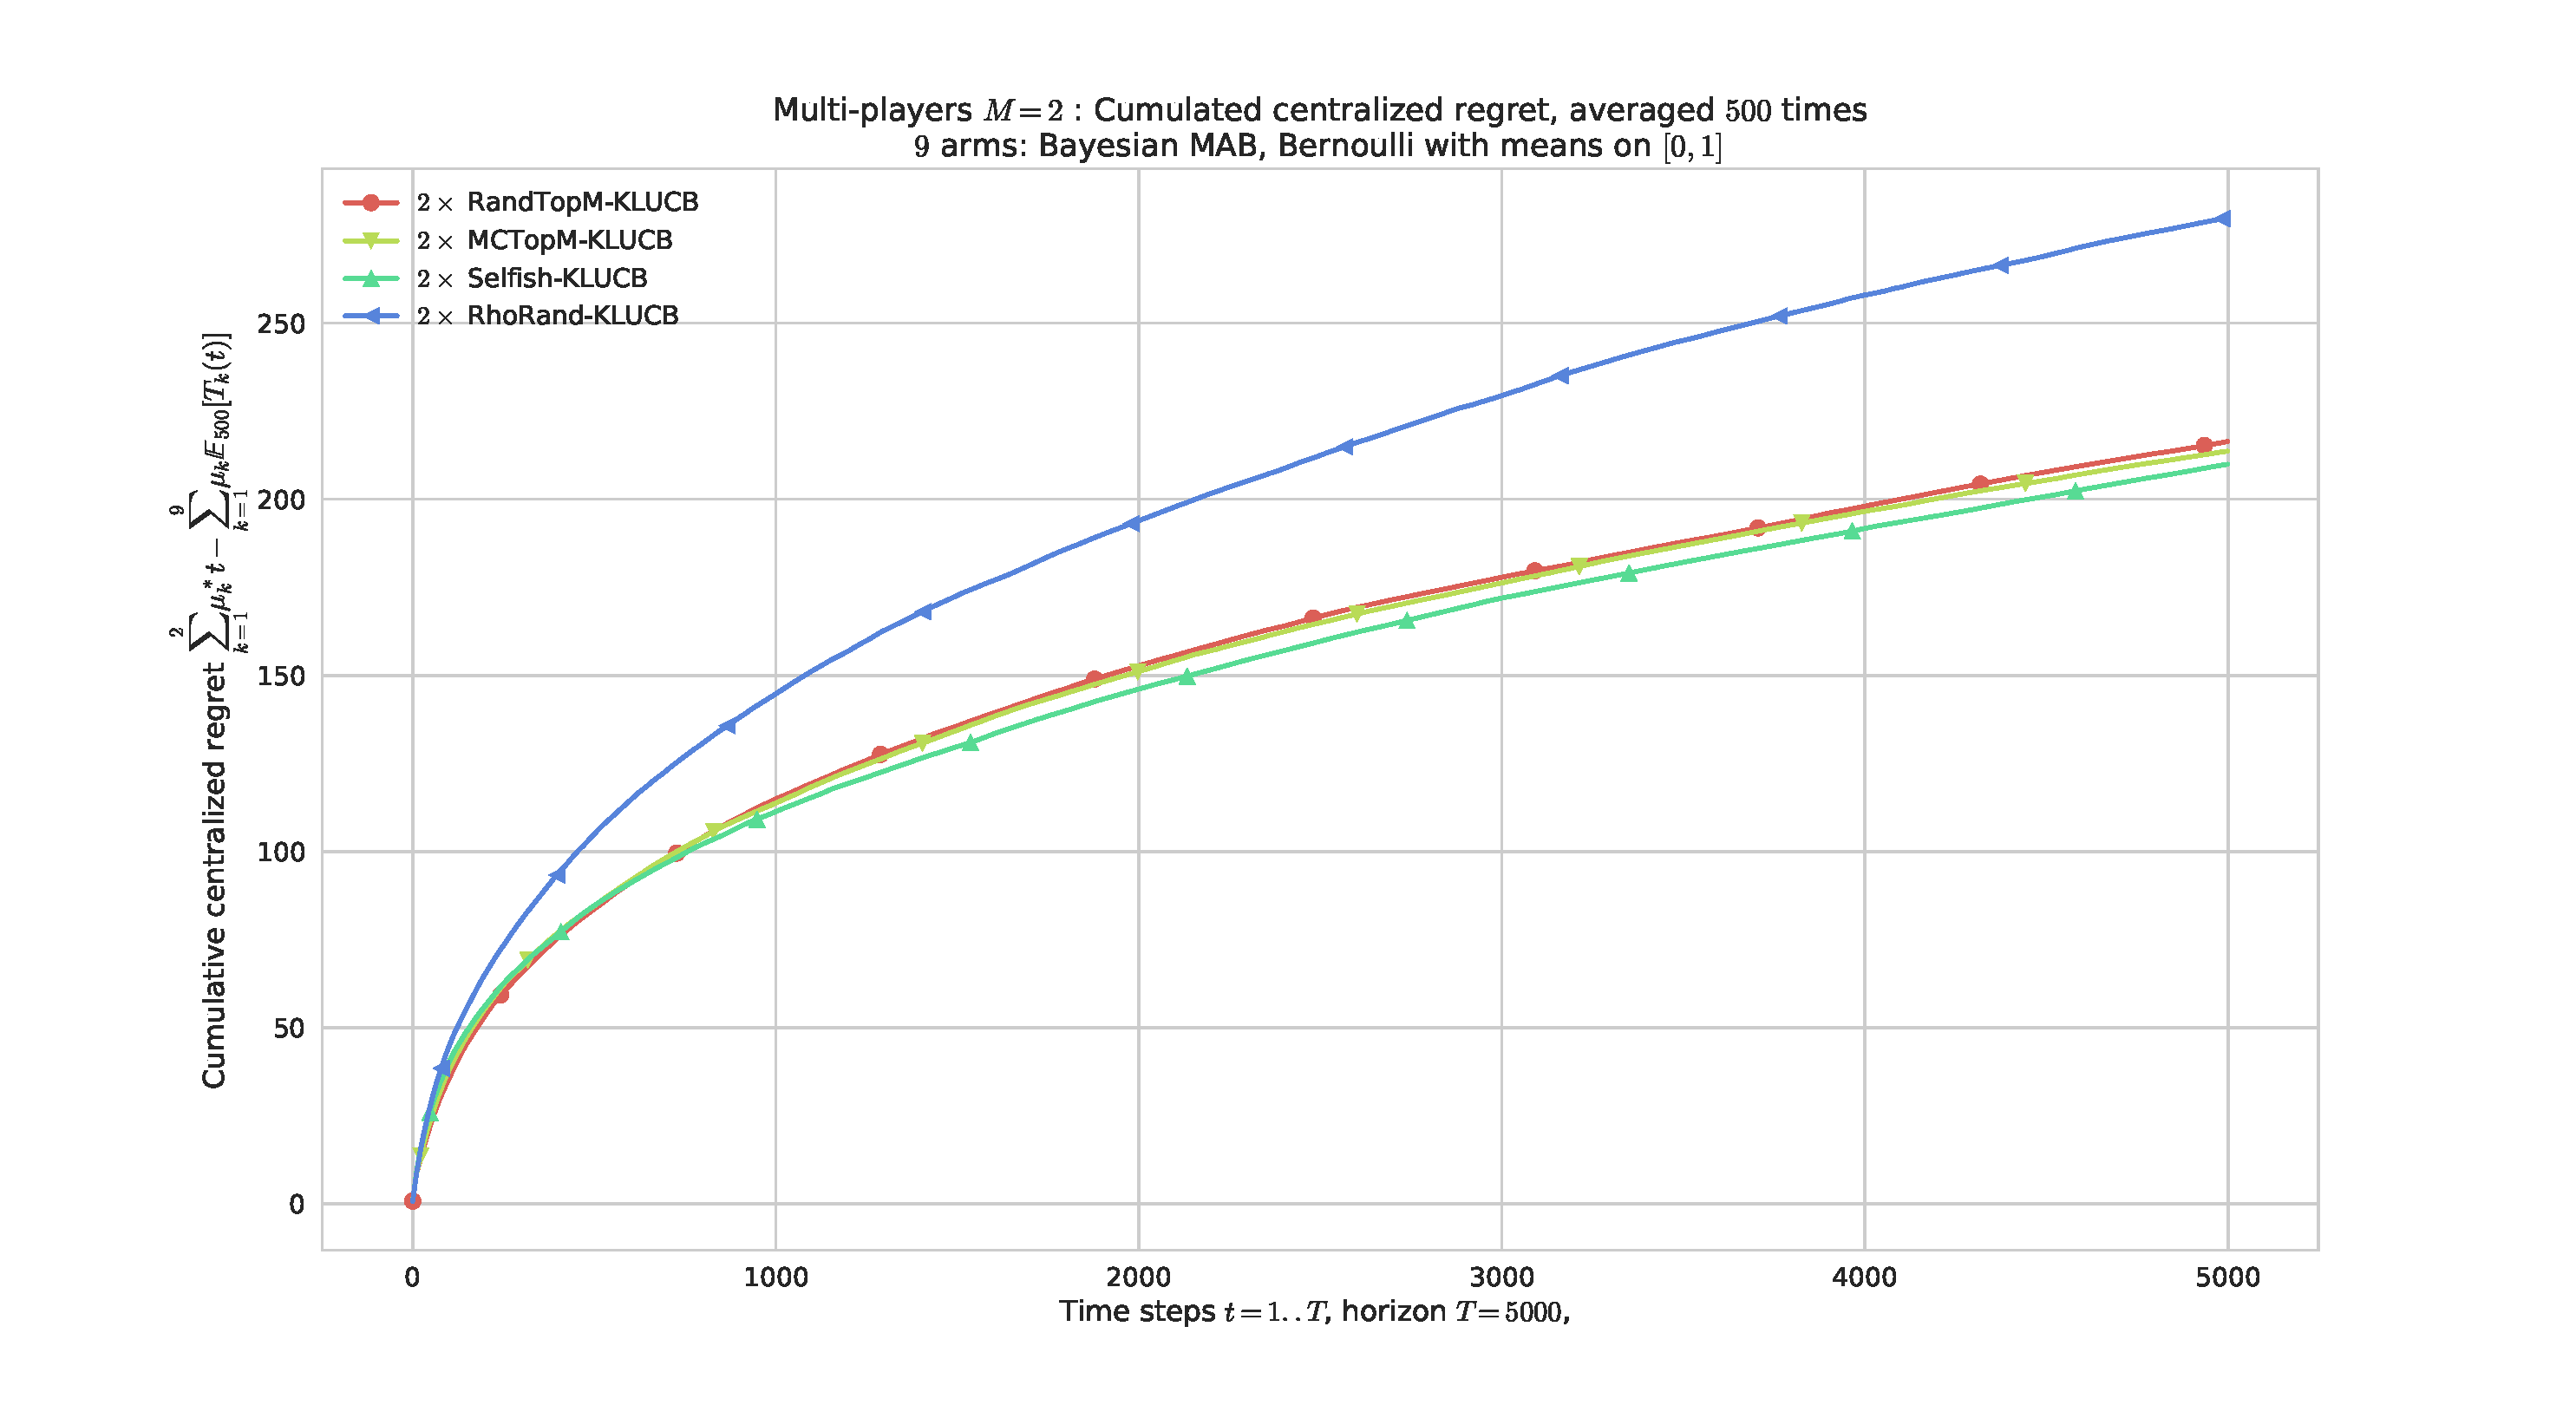
\includegraphics[width=1.00\textwidth]{MP__K9_M2_T5000_N500__4_algos/all_RegretCentralized____env1-1_3251433209347345969.pdf}
  % \end{subfigure}
  % % ~
  % \begin{subfigure}[!h]{0.49\textwidth}
    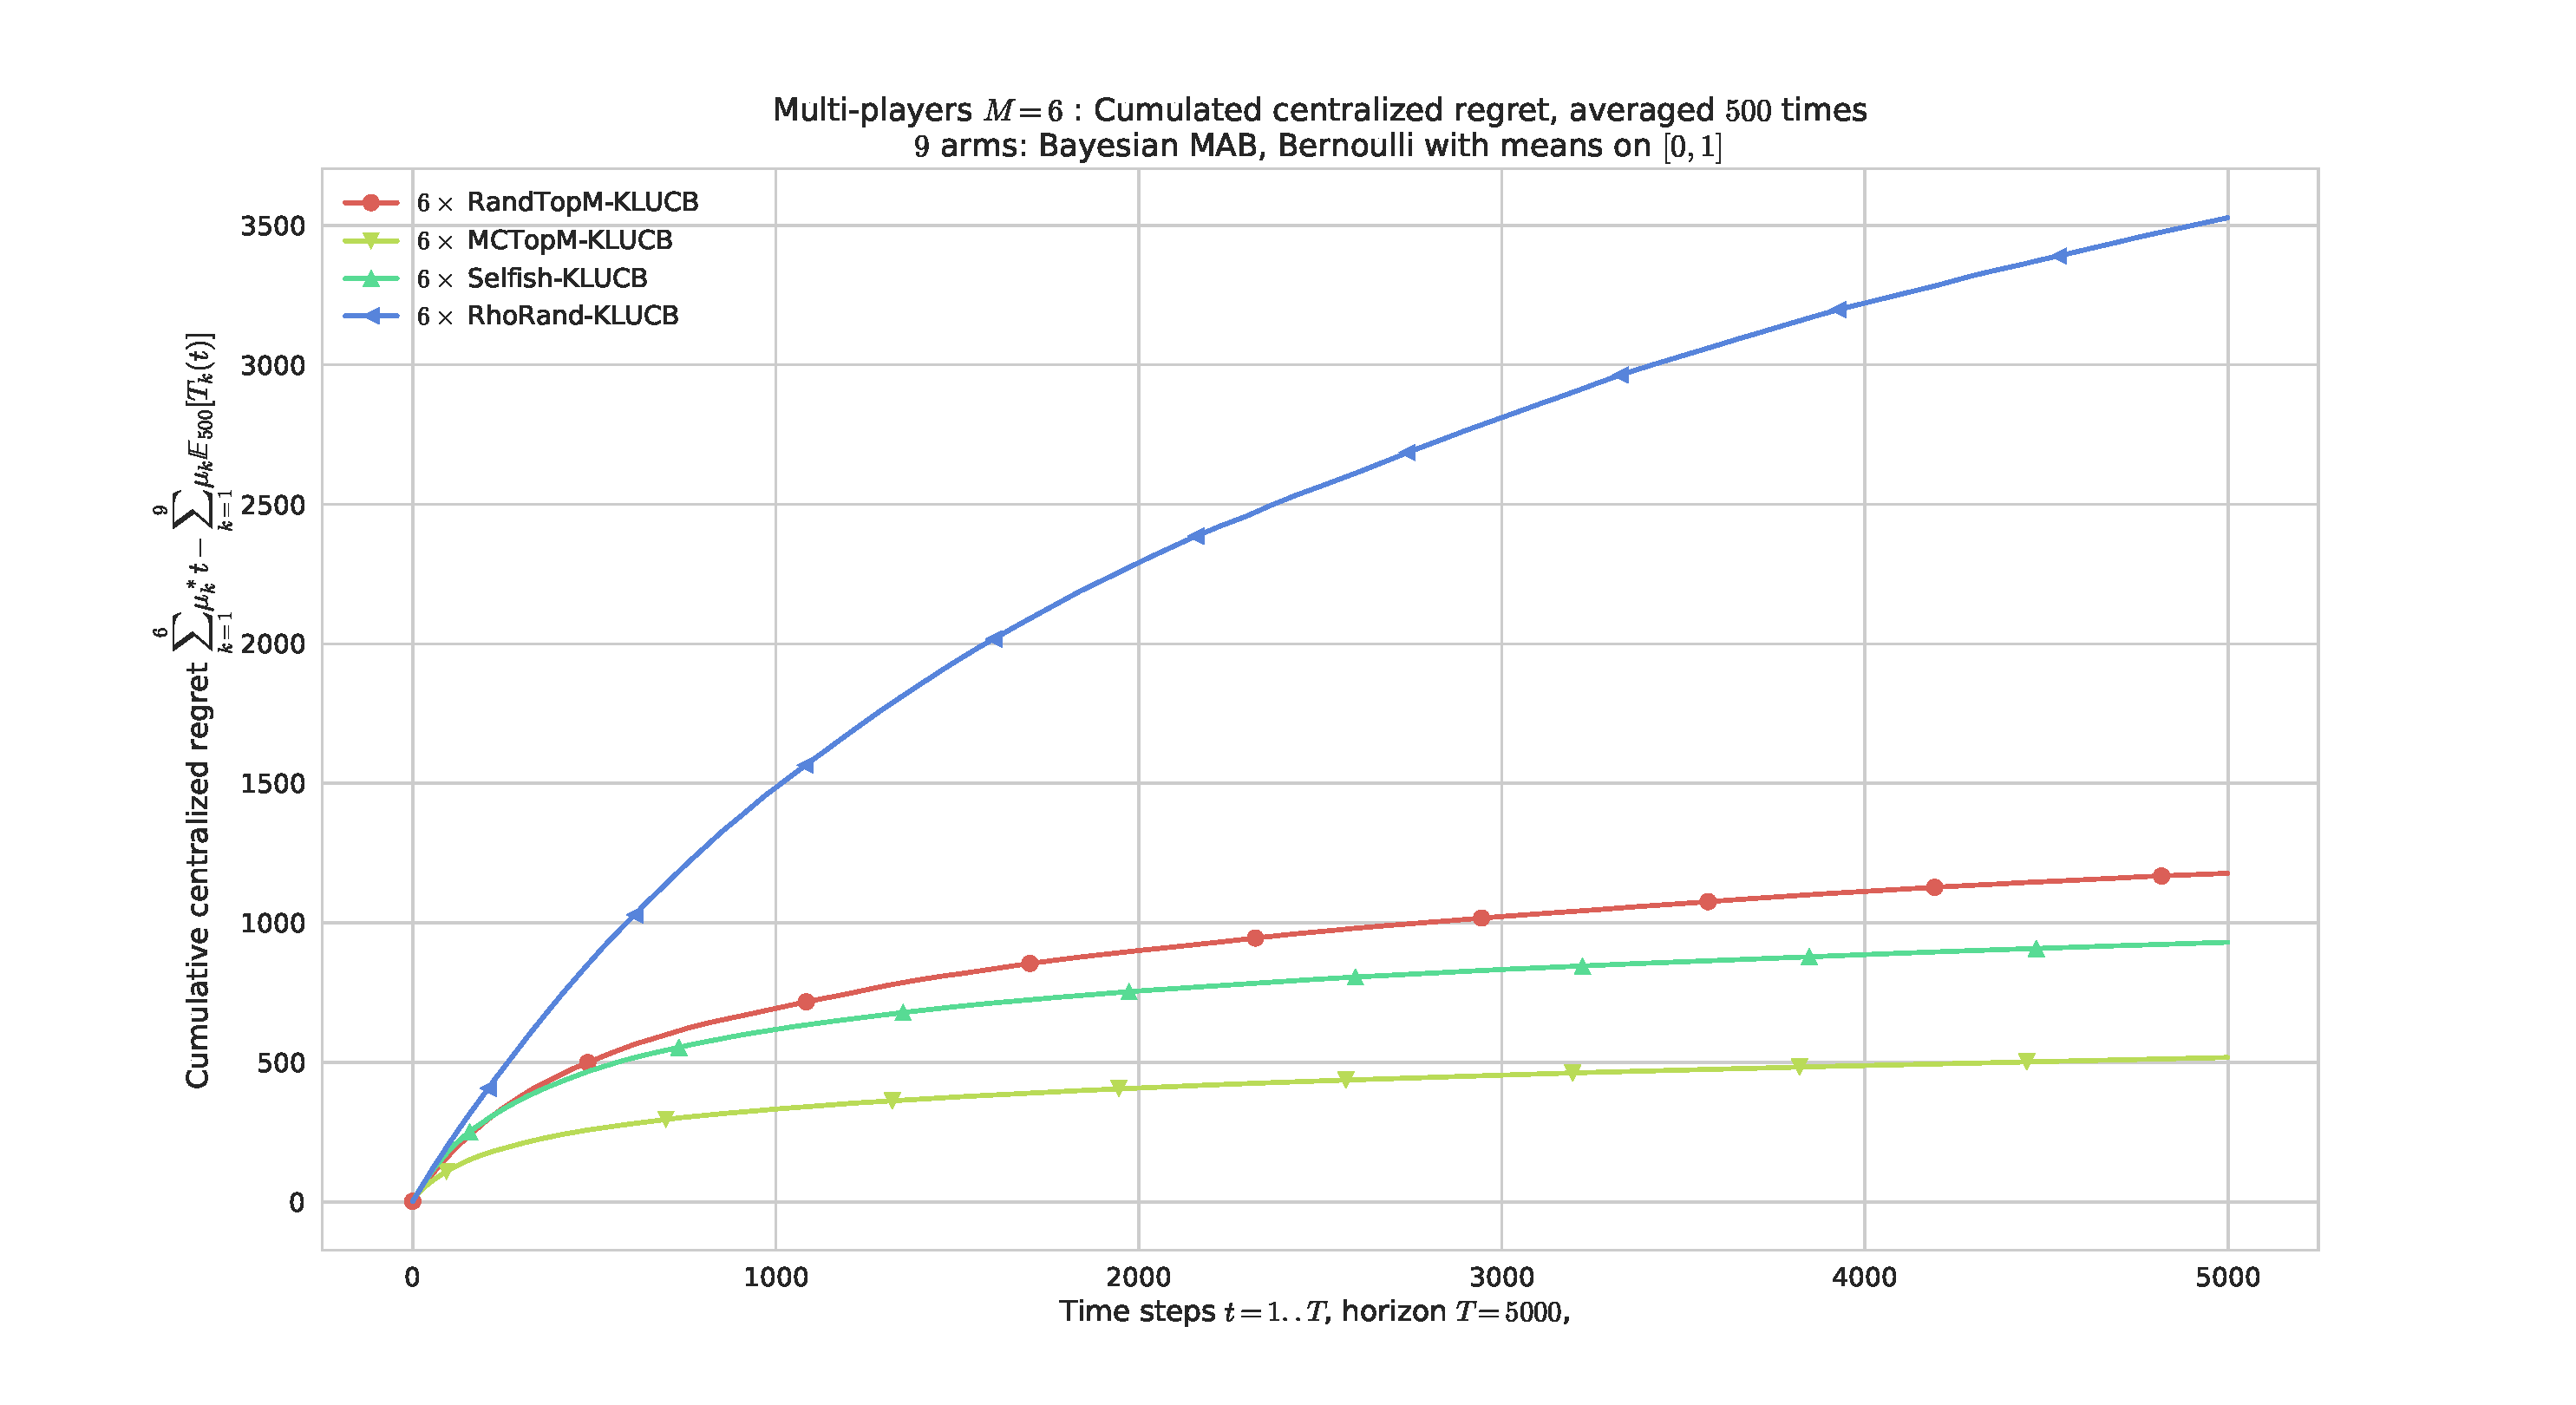
\includegraphics[width=1.00\textwidth]{MP__K9_M6_T5000_N500__4_algos/all_RegretCentralized____env1-1_8318947830261751207.pdf}
  % \end{subfigure}
  \caption[Regret for $M=6$ players, $K=9$ arms, horizon $T=5000$, against $500$ problems $\boldsymbol{\mu}$ uniformly sampled]{Regret for $M=6$ players, $K=9$ arms, horizon $T=5000$, against $500$ problems $\boldsymbol{\mu}$ uniformly sampled in $[0,1]^K$. \rhoRand{} (top \textcolor{blue}{blue} curve) is outperformed by the other algorithms (and the gain increases with $M$). \MCTopM{} (bottom \textcolor{gold}{yellow}) outperforms all the other algorithms is most cases.}
  % \label{fig:5:MP__K9_M2-6_T5000_N500__4_algos__all_RegretCentralized__BayesianProblems}
  \label{fig:5:MP__K9_M6_T5000_N500__4_algos__all_RegretCentralized__BayesianProblems}
  % \vspace*{-15pt}  % XXX remove if problem
\end{figure}



% Dynamic settings, when $M$ can change in time,
% were considered in the analysis of both
In the presence of sensing (observation model \modeldeux), we also compared our algorithms to  %multi-player multi-armed bandits algorithms
with \MEGA{} \citep{Avner15} and \MusicalChair{} \citep{Rosenski16}. Yet these two algorithms were found hard to use efficiently in practice and we show in
% that were also proposed
%
Figure~\ref{fig:5:MP__K9_M3_T123456_N100__8_algos} that they perform poorly in comparison to \rhoRand, \RandTopM{} and \MCTopM.
%
\MEGA{} needs a careful tuning of \emph{five} parameters ($c$, $d$, $p_0$, $\alpha$ and $\beta$) to attain reasonable performances. No good guideline for tuning them is provided and using cross validation, as suggested,
can be considered out of the scope of online sequential learning.
%In practice, on a fixed instance, the authors do not indicate how to select the parameters, even with a perfect knowledge of the parameters ($\boldsymbol{\mu}$ and $T$).
%
\MusicalChair{} consists of a random exploration phase of length $T_0$ after which the players quickly converge to orthogonal strategies targeting the $M$ best arms. With probability $1-\delta$, its regret is proved to be ``constant'' (of order $\log(1/\delta)$). The theoretical minimal value for $T_0$ depends on $\delta$, on the horizon $T$ and on a lower bound $\epsilon$ on the gap $\Delta = \mu^*_M - \mu^*_{M+1}$, and the practical tuning is hard too. %% which are both unavailable in our setting.



\begin{figure}[!h]
  \centering
  % \begin{subfigure}[!h]{0.85\textwidth}
    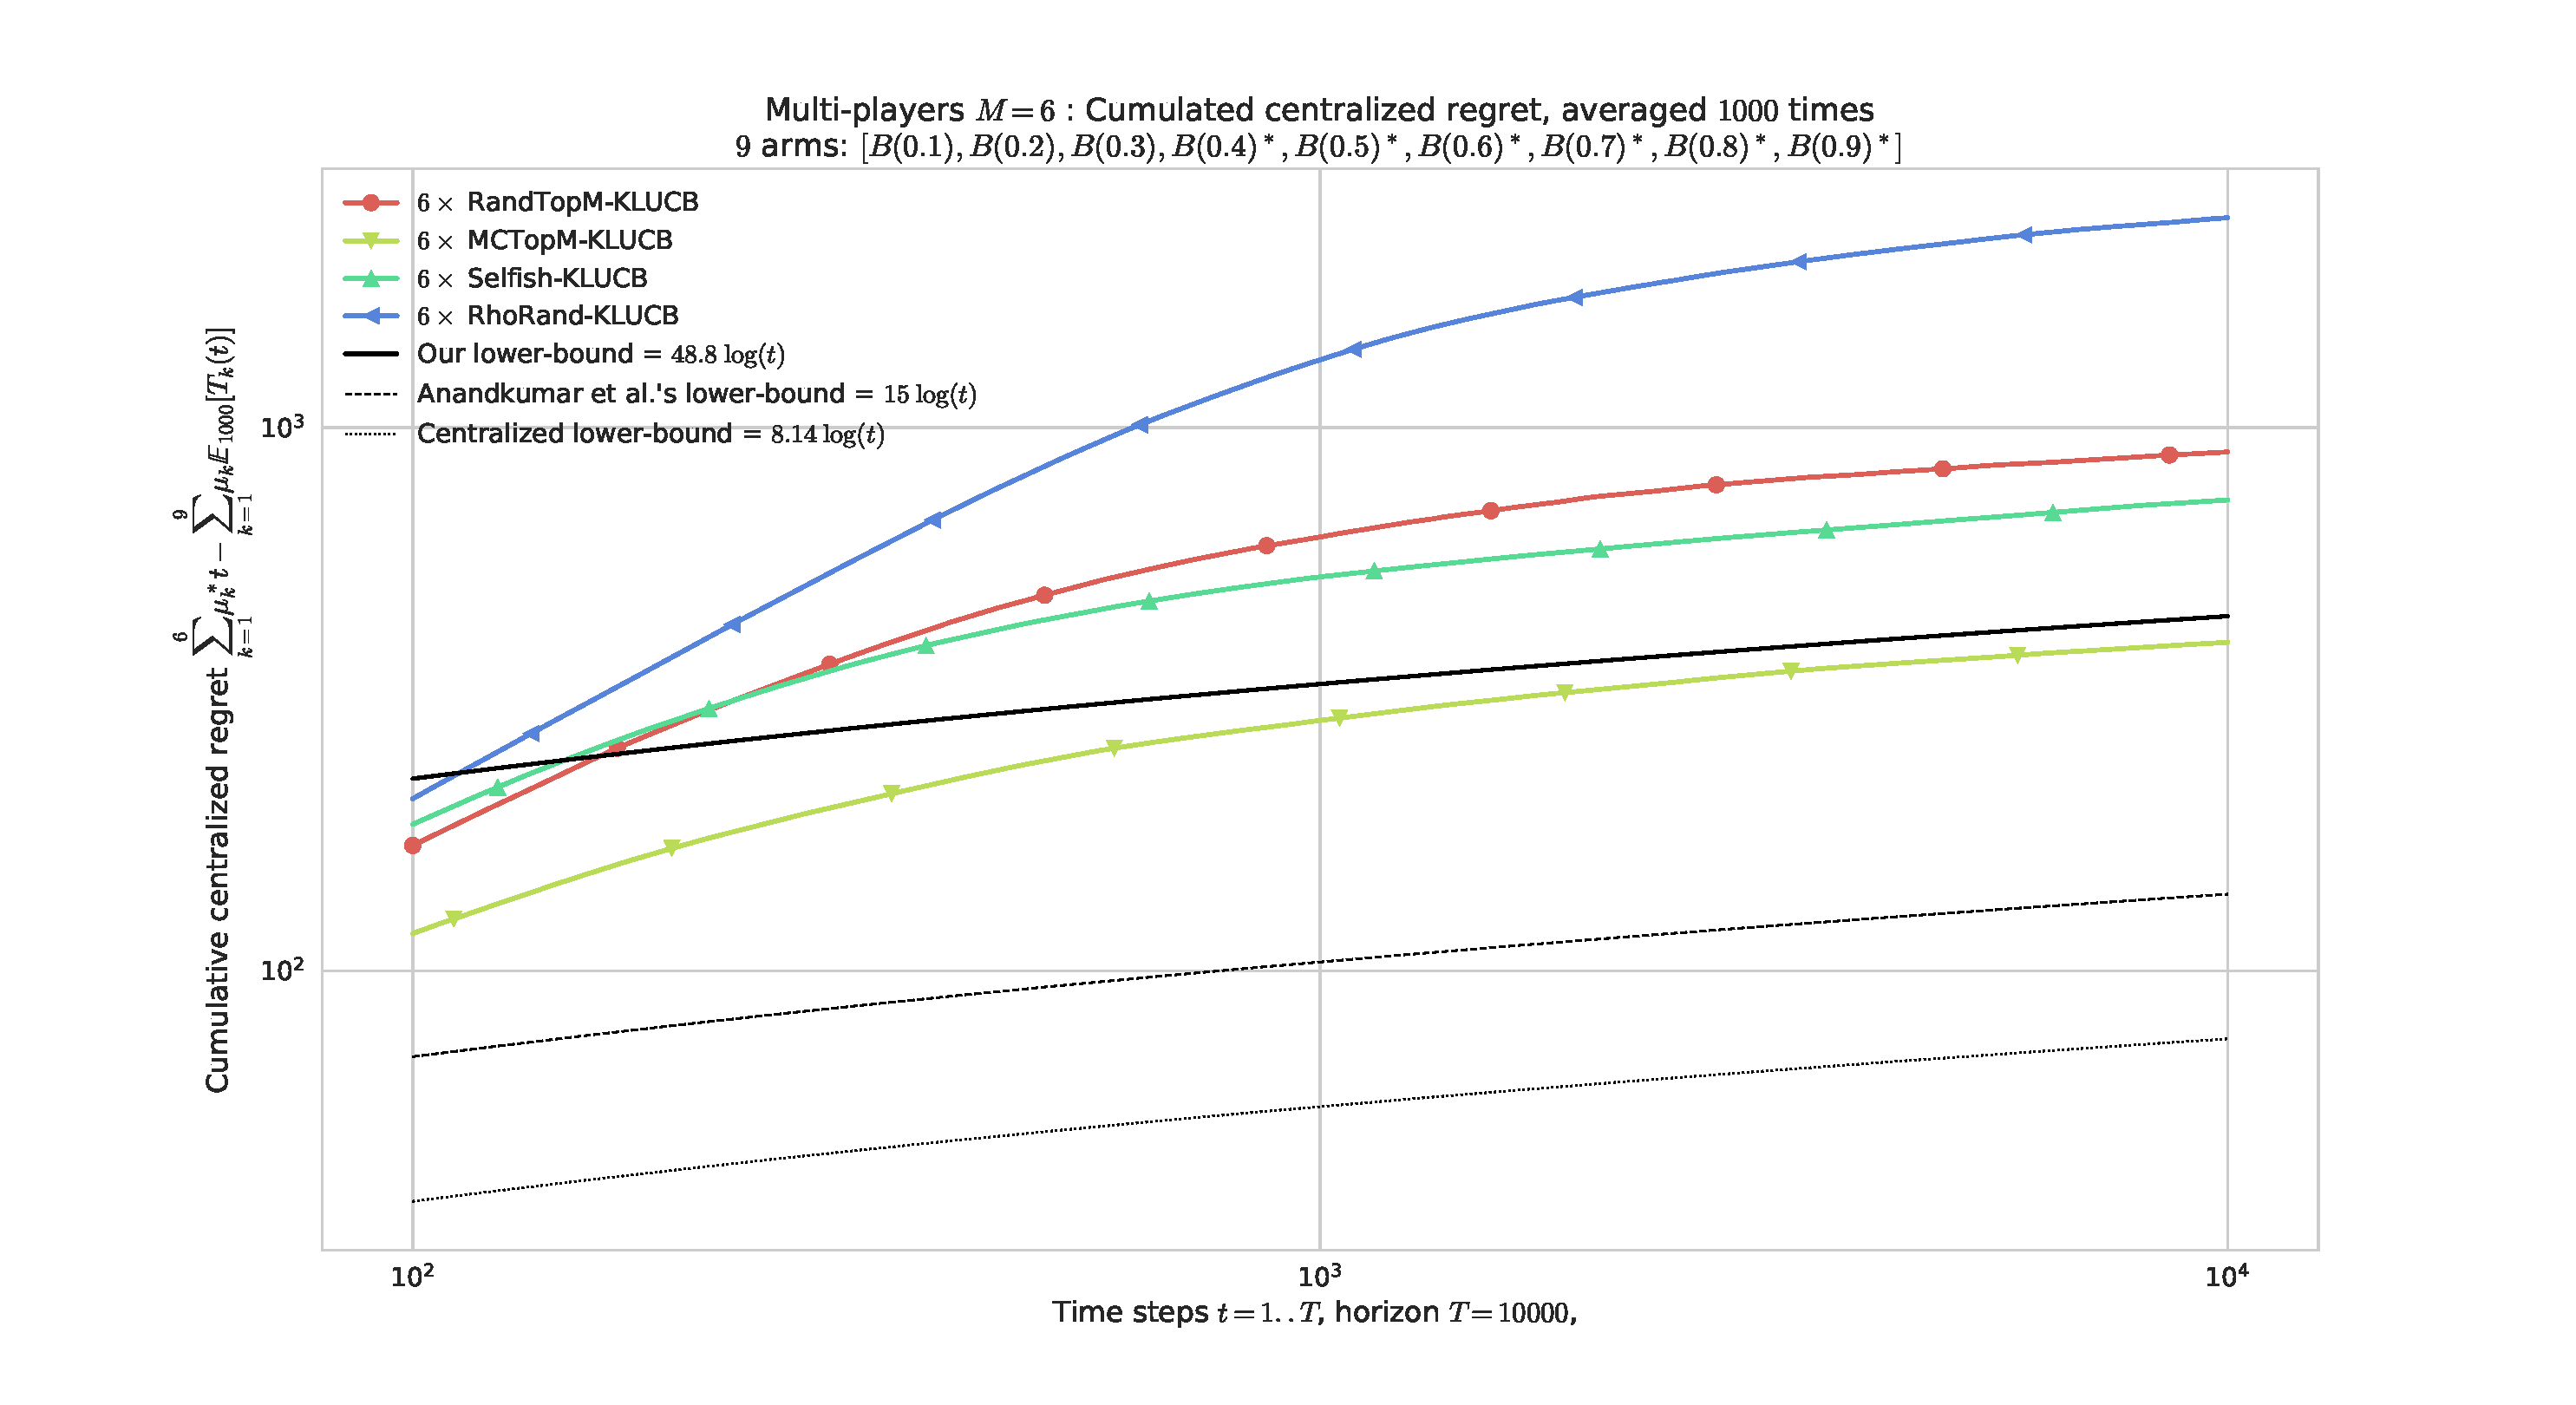
\includegraphics[width=1.00\textwidth]{MP__K9_M6_T10000_N1000__4_algos/all_RegretCentralized_loglog____env1-1_8200873569864822246.pdf}
  % \end{subfigure}
  % ~
  % \begin{subfigure}[!h]{0.85\textwidth}
    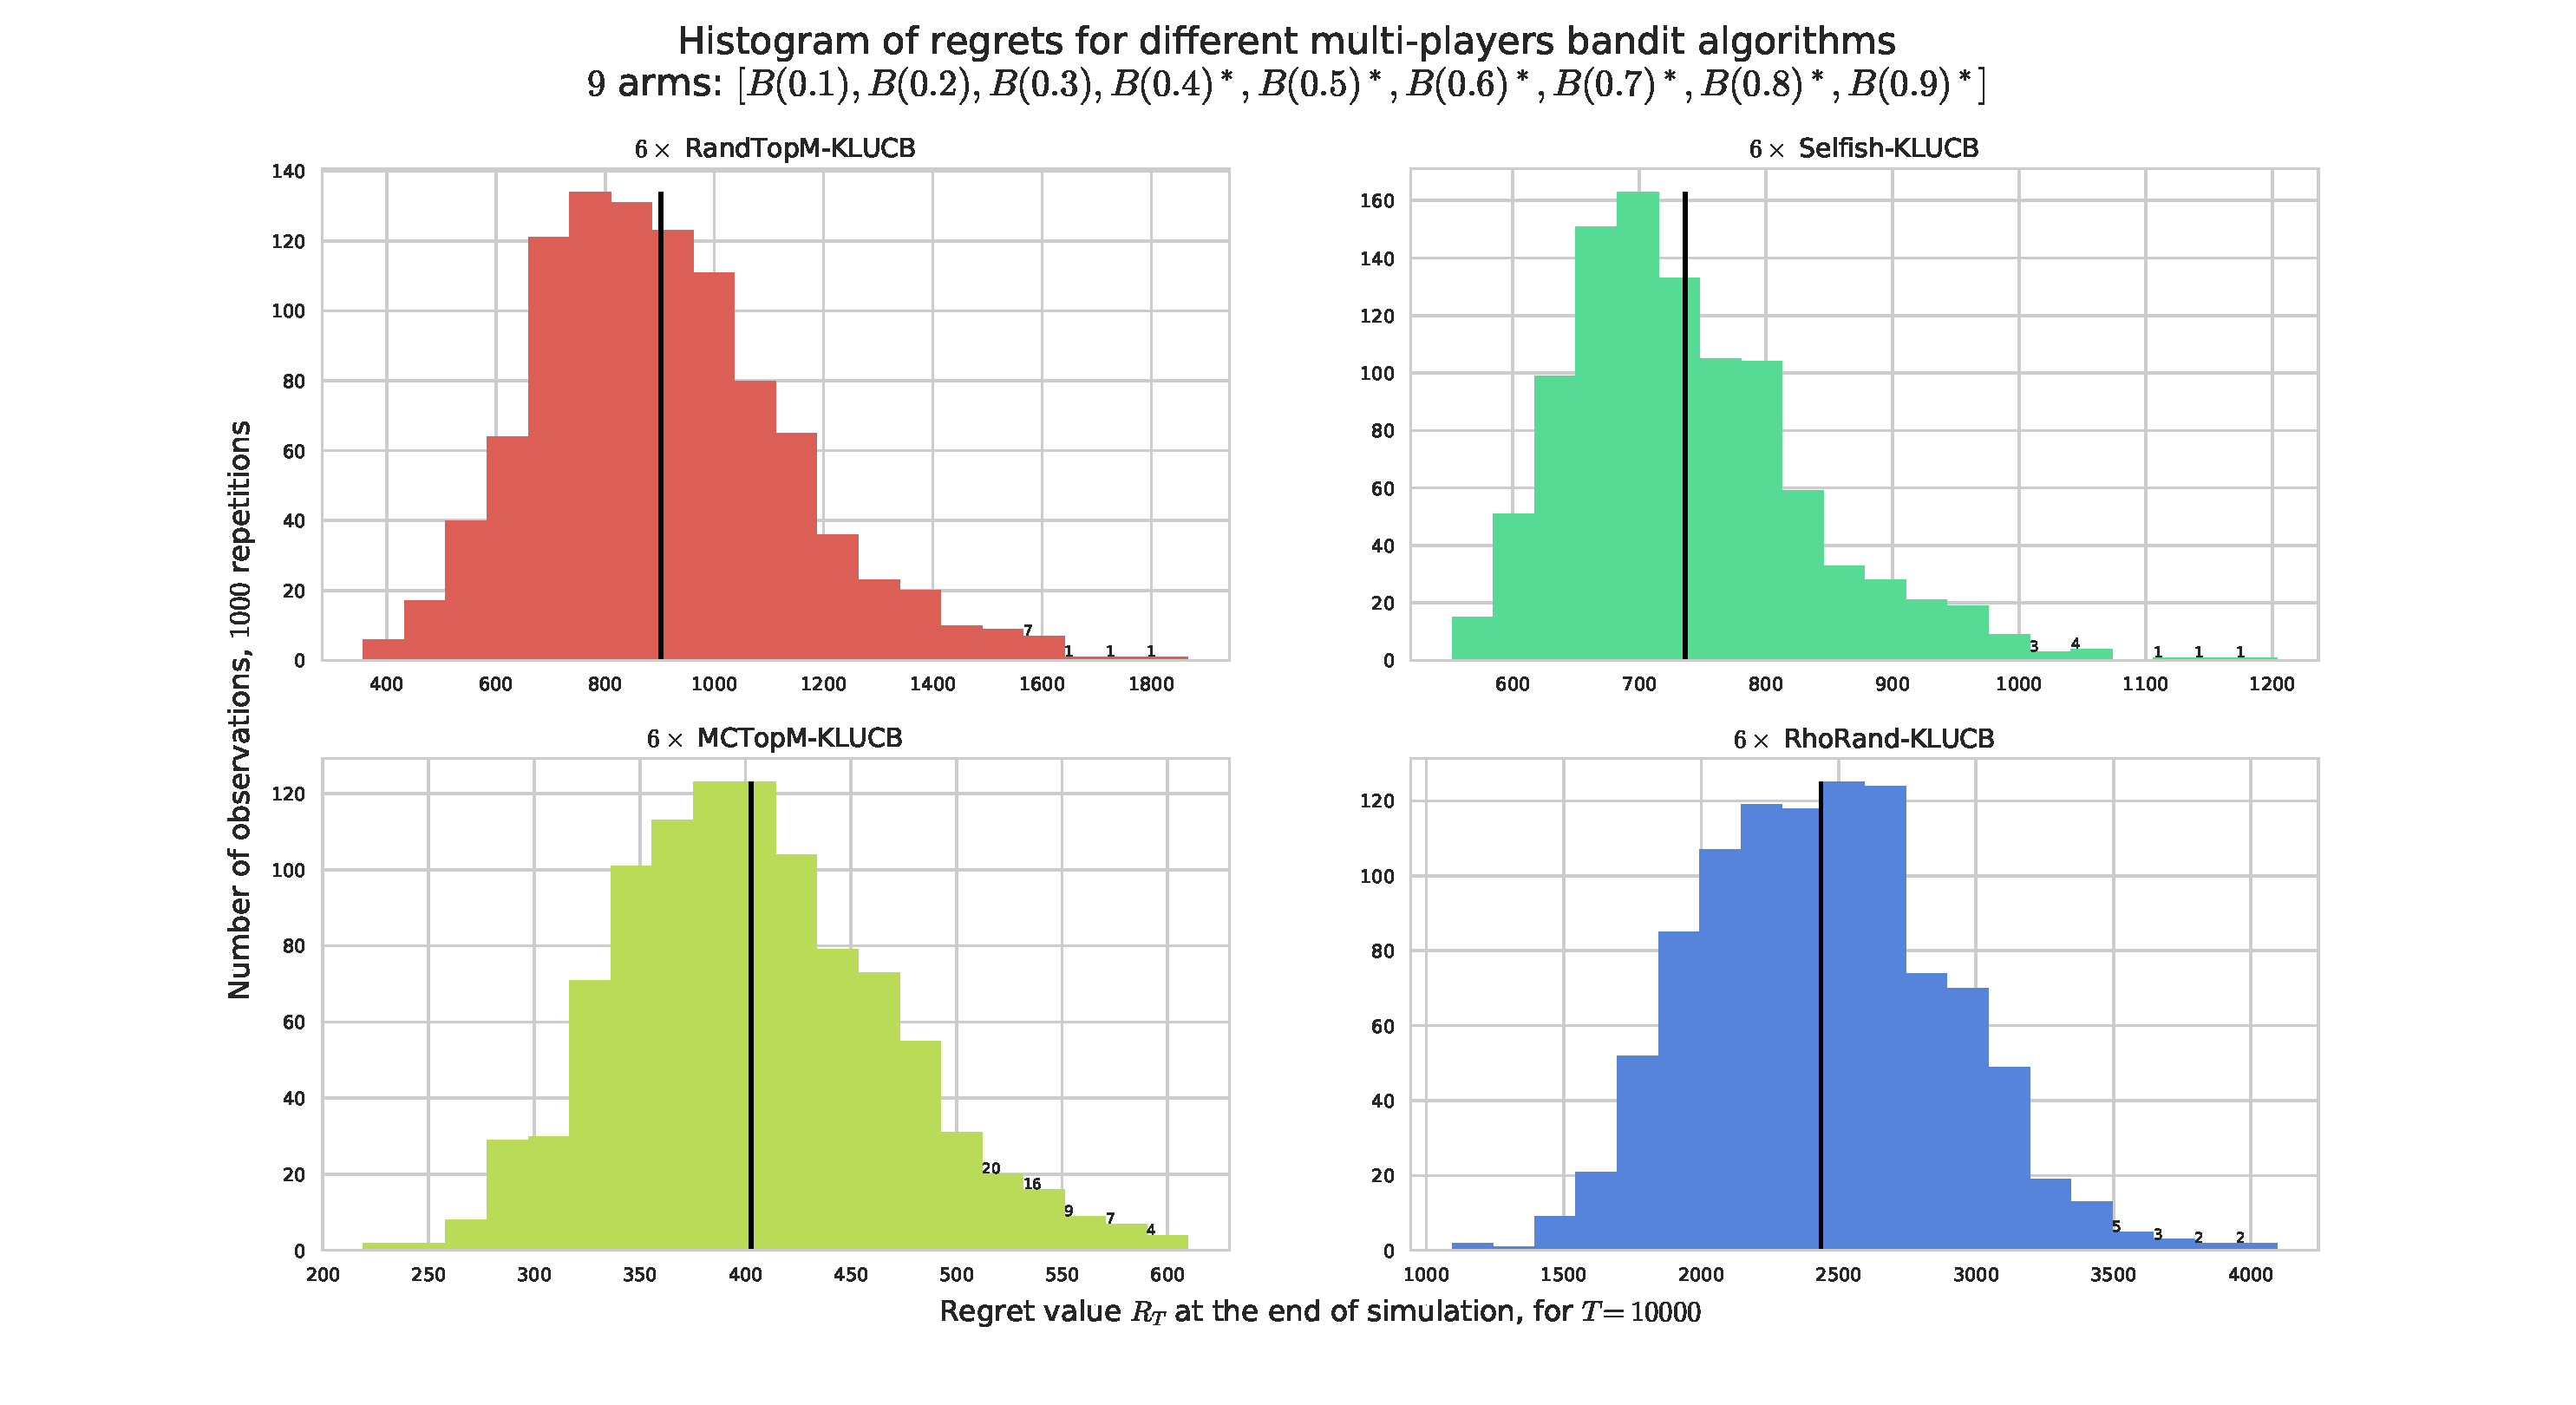
\includegraphics[width=1.00\textwidth]{MP__K9_M6_T10000_N1000__4_algos/all_HistogramsRegret____env1-1_8200873569864822246.pdf}
  % \end{subfigure}
  \caption[Regret for $M=6$ players for $K=9$ arms, horizon $T=5000$, for $1000$ repetitions on a fixed problem]{Regret (in log-log scale), for $M=6$ players for $K=9$ arms, horizon $T=5000$, for $1000$ repetitions on problem $\boldsymbol{\mu}=[0.1,\dots,0.9]$. \RandTopM{} (\textcolor{gold}{yellow} curve) outperforms \Selfish{} (\textcolor{darkgreen}{green}), both clearly outperform \rhoRand. The regret of \MCTopM{} is logarithmic, empirically with the same slope as the lower bound. The $x$ axis on the regret histograms have different scale for each algorithm.}
  \label{fig:5:MP__K9_M6_T10000_N1000__4_algos}
\end{figure}




% -----------------------------------------------------------------
\section{Theoretical elements}
\label{sec:5:upperbounds}
% -----------------------------------------------------------------


Section~\ref{sub:5:UpperBoundSelections} gives
an asymptotically optimal analysis of the expected number of sub-optimal draws
for \RandTopM, \MCTopM{} and \rhoRand{} combined with \klUCB{} indices,
and Section~\ref{sub:5:UpperBoundCollisions} proves that the number of  collisions, hence the regret of \MCTopM{} are also logarithmic.
%
Section~\ref{sub:5:SelfishFails} shortly discusses a disappointing result regarding \Selfish{}, with more insights provided in Appendix~\ref{app:5:SelfishFails}.


% -----------------------------------------------------------------
\subsection{Common analysis for \RandTopM- and \MCTopM-\klUCB{}}\label{sub:5:UpperBoundSelections}

Lemma~\ref{lem:5:SubOptimalSelections} gives a finite-time upper bound on the expected number of draws of a sub-optimal arm $k$ for any player $j$, that
holds for both \RandTopM-\klUCB{} and \MCTopM-\klUCB.
Our improved analysis also applies to \rhoRand{}.
Explicit expressions for $C_{\boldsymbol{\mu}}$, $D_{\boldsymbol{\mu}}$ can be found in the proof given in Appendix~\ref{proof:5:SubOptimalSelections}.

\begin{lemma}\label{lem:5:SubOptimalSelections}
  For any $\boldsymbol{\mu}\in\cP_M$,
  if player $j\in\{1,\dots,M\}$ uses the \RandTopM-, \MCTopM- or \rhoRand-\klUCB{}
  decentralized policy with exploration function $f(t) = \log(t) + 3 \log\log(t)$,
  then for any sub-optimal arm $k \in \Mworst$, there exists two problem depend constants $C_{\boldsymbol{\mu}}$, $D_{\boldsymbol{\mu}}$ such that
  % %
  % \hfill{}
  % (Proved in Appendix~\ref{proof:5:SubOptimalSelections})
  \begin{equation}\label{eq:5:SubOptimalSelections}
      \E_{\mu}[T_k^j(T)] \leq \frac{\log(T)}{\kl(\mu_k,\mu_{M}^*)}+ C_{\boldsymbol{\mu}} \sqrt{\log(T)} + D_{\boldsymbol{\mu}}\log\log(T) + 3M + 1.
  \end{equation}
\end{lemma}

It is important to notice that the leading constant in front of $\log(T)$ is the same as in the constant featured in Equation~\eqref{eq:5:LBDraws} of Theorem~\ref{thm:5:BetterLowerBound}. This result proves that the lower bound on sub-optimal selections is asymptotically matched for the three considered algorithms. This is a strong improvement in comparison to the previous state-of-the-art results
\citep{Zhao10,Anandkumar11}.


% -----------------------------------------------------------------

% For \rhoRand-\klUCB{} we used results from \cite{Anandkumar11}
% to control the number of collisions on sub-optimal arms.
% %
% For \RandTopM-\klUCB{} we have a better control over the number of collisions,
% and as expected we can bound it by a logarithmic term with a much smaller constant.
% The \RandTopM{} policy was indeed designed to be more ``conservative'' in its dynamics
% in order to reduce the number of collisions caused by a player who changes from his current chosen arm
% in an orthogonal configuration.

% For \rhoRand, \cite{Anandkumar11} essentially proved on one hand that conditionnaly to a certain ``good'' event
% (all players have a correct ordering of all the $M$ best arms)
% proved to happen with high probability,
% the total number of collisions is upper bounded asymptotically by ${2 M - 1 \choose M}$,
% which is constant but grows very quickly as $M$ grows.
% And on the other hand, they proved that the total number of steps when this event is violated is $\bigO{\log T}$, with large constants in the asymptotic notation.


As announced, Lemma~\ref{lem:5:elementaryLemma_RandTopM_MCTopM} controls
the number of switches of arm that are due to the current arm leaving $\TopM(t)$,
for both \RandTopM{} and \MCTopM{}. It essentially proves that Lines~$3$-$5$ in Algorithm~\ref{algo:5:MCTopM} (when a new arm is sampled from the non-empty subset of $\TopM(t)$)
happen a logarithmic number of times. The proof of this result is given in Appendix~\ref{proof:5:elementaryLemma_RandTopM_MCTopM}.

\begin{lemma}\label{lem:5:elementaryLemma_RandTopM_MCTopM}
  For any $\boldsymbol{\mu}\in\cP_M$,
  any player $j \in \{1, \dots, M\}$ using
  \RandTopM- or \MCTopM-\klUCB,
  and any arm $k$,
  it holds that
  \begin{equation*}
    \sum_{t=1}^T
    \Pr\left(A^j(t)=k, k\notin \TopM(t)\right)
    = \left(\sum_{k', \mu_{k'} < \mu_k}\frac{1}{\kl(\mu_k,\mu_{k'})} + \sum_{k', \mu_{k'} > \mu_k}\frac{1}{\kl(\mu_{k'},\mu_{k})}\right) \log(T) + o(\log(T)).
  \end{equation*}
\end{lemma}


% -----------------------------------------------------------------
\subsection{Regret analysis of \MCTopM-\klUCB}\label{sub:5:UpperBoundCollisions}

For \MCTopM, we are furthermore able to obtain a logarithmic regret upper bound, by proposing an original approach to control the number of collisions under this algorithm.
First, we can bound the number of collisions by the number of collisions for players not yet ``fixed on their arms'' ($\overline{s^j(t)}$),
that we can then bound by the number of changes of arms
(\cf{} proof in Appendix~\ref{proof:5:collisionsMCTopM}).
%
An interesting consequence of the proof of this result is that
it also bounds the number of \emph{switches of arms}, $\sum_{t=1}^T \Pr(A^j(t+1) \neq A^j(t))$,
and this additional guarantee was never clearly stated for previous state-of-the-art works, like \rhoRand.
Even though minimizing switching was not a goal\footnote{Introducing \emph{switching costs}, like it was done in previous works, \eg, \cite{Koren17}, could be an interesting future work.},
this guarantee is interesting for Cognitive Radio applications,
where switching arms means reconfiguring a radio hardware, an operation that costs energy.
%and thus an algorithm guaranting a small number of switches is interesting.

\begin{lemma}\label{lem:5:collisionsMCTopM}
  For any $\boldsymbol{\mu}\in\cP_M$,
  if all players use the
  \MCTopM-\klUCB{} decentralized policy,
  and $M \leq K$,
  then the total average number of collisions (on all arms)
  is upper-bounded by
  \hfill{}
  (Proved in Appendix~\ref{proof:5:collisionsMCTopM})
  \begin{equation}
    \E_{\mu}\left[\sum_{k=1}^K \cC_k(T)\right]
    \leq M^2\left(2 M + 1\right) \left(\sum_{a,b=1,\dots,K,\;\mu_a < \mu_b} \frac{1}{\kl(\mu_a,\mu_b)}\right) \log(T) + \smallO{\log T}.
  \end{equation}
\end{lemma}

Note that this bound is in $\bigO{M^3}$,
which significantly improves the $\bigO{M{2M-1 \choose M}}$ proved by \cite{Anandkumar11} for \rhoRand. It is worse than the $\bigO{M^2}$ proved by \cite{Rosenski16} for \MusicalChair{}. %, due to our trick of focusing on collisions for non-sitted players.
However, unlike \MusicalChair{} our algorithm does not need the knowledge of $\mu^*_{M}-\mu^*_{M+1}$.


% -----------------------------------------------------------------
% \subsection{Logarithmic Regret for \MCTopM}\label{sub:5:Regret}

Now that the sub-optimal arms selections and the collisions
are both proved to be at most logarithmic in Lemmas~\ref{lem:5:SubOptimalSelections} and \ref{lem:5:collisionsMCTopM},
it follows from our regret decomposition (Lemma~\ref{lem:5:DecompositionRegret}) together with Lemma~\ref{lem:5:1stUpperBound} that the regret of \MCTopM-\klUCB{} is logarithmic. More precisely, one obtains a finite-time problem-depend upper bound on the regret of this algorithm.

\begin{theorem}\label{thm:5:LogarithmicRegret_MCTopMklUCB}
  If all $M$ players use
  \MCTopM-\klUCB, and $M \leq K$,
  then for any problem $\boldsymbol{\mu} \in \cP_M$,
  there exists a problem dependent constant $G_{M,\boldsymbol{\mu}}$, such that
  the regret satisfies:
  \begin{equation}\label{eq:5:LogarithmicRegret_MCTopMklUCB}
    R_T(\boldsymbol{\mu}, M, \rho) \leq G_{M,\boldsymbol{\mu}} \log(T) + \smallO{\log T}.
  \end{equation}
\end{theorem}


% -----------------------------------------------------------------
\subsection{Discussion on \Selfish} \label{sub:5:SelfishFails}

The analysis of \Selfish{} is harder, but we tried our best to obtain some understanding of the behavior of this algorithm, that seems to be doing surprisingly well in many contexts, as in our experiments with $K=9$ arms and in extensive experiments not reported in this Section. However, a disappointing result is that we found simple problems, usually with small number of arms, for which the algorithm may fail. For example with $M=2$ or $M=3$ players competing for $K=3$ arms,
with means $\boldsymbol{\mu} = [0.1, 0.5, 0.9]$, the histograms in Figure~\ref{fig:5:selfish_fail1} suggests that with a small probability, the regret $R_T$ of \Selfish-\klUCB{} can be very large. We provide a discussion in Appendix~\ref{app:5:SelfishFails} about when such situations may happen, including a conjectured (constant, but small) lower bound on the probability that \Selfish{} experience collision almost at every round. This result would then prevent \Selfish{} from having a logarithmic regret. However, it is to be noted that the lower bound of Theorem~\ref{thm:5:BetterLowerBound} does not apply to the censored observation model \modeltrois{} under which \Selfish{} operates, and it is not known yet whether logarithmic regret is at all possible.



% -----------------------------------------------------------------
\section{Conclusion and future work}
\label{sec:5:conclusion}
% -----------------------------------------------------------------

To summarize, we presented three variants of Multi-Player Multi-Arm Bandits,
with different level of feedback being available to the decentralized players, under which we proposed efficient algorithms.
For the two easiest models --with sensing--, our theoretical contribution improves both the state-of-the-art upper and lower bounds on the regret. In the absence of sensing, we also provide some motivation for the practical use of the interesting \Selfish{} heuristic, a simple index policy based on hybrid indices that are directly taking  into account the collision information.

This work suggests several interesting further research directions. First, we want to investigate the notion of \emph{optimal algorithms} in the decentralized multi-player model with sensing information. So far we provided the first matching upper and lower bound on the expected number of sub-optimal arms selections, which suggests some form of (asymptotic) optimality. However, sub-optimal draws turn out not be the dominant terms in the regret, both in our upper bounds and in practice, thus an interesting future work is to identify some notion of \emph{minimal number of collisions}. Second, it remains an open question to know if a simple decentralized algorithm can be as efficient as \MCTopM{} without knowing $M$ in advance, or in dynamic settings (when $M$ can change in time). We shall start by proposing variants of our algorithm that are inspired by the \rhoRandEst{} variant of \rhoRand{} proposed by \cite{Anandkumar11}.
Finally, we want to strengthen the guarantees obtained in the absence of sensing, that is to know whether logarithmic regret is achievable and to have a better analysis of the \Selfish{} approach.  Indeed, in most cases, it performs comparably to \RandTopM{} even with limited feedback and without knowing the number of players $M$, which makes it a good candidate for applications to Internet of Things networks.


% -----------------------------------------------------------------


% \paragraph{Acknowledgments}
% Thanks to Odalric-Ambrym Maillard at Inria Lille for useful discussions, and thanks to Christophe Moy at University Rennes 1.

\paragraph{A note on the simulation code}
The page \texttt{SMPyBandits.GitHub.io/MultiPlayers.html} explains how to reproduce the experiments used for this Section.

% biblio usually before the supplementary material
% \bibliography{mpBandits}
